
\chapter{Mapping the T-cell transcriptional landscape: can we utilise  currently available clustering techniques  to define a module map?} % Main chapter title

\label{Chapter4} % For referencing the chapter elsewhere, use \ref{Chapter1} 

%----------------------------------------------------------------------------------------
\section{Overview}

This Chapter details the results of reclustering of the ImmGen T cell dataset (for an overview of the data please see Chapter \ref{Chapter1}. Three clustering algorithms were implemented, specifically WGCNA, Hclust and K-means. All three methodologies are described in Chapter \ref{Chapter3}. The primary aim of this work is to compare and contrast how different algorithms behave when tasked with clustering the same data and to attempt some quantification of the biological relevance of the module sets produced in each case. The following sections summarise some of the key steps/decisions taken during clustering as well as comparing how the output modules from each algorithm relate to the original Coarse modules published by the ImmGen consortium. 

\section{Weighted Gene Correlation Network Analysis (WGCNA)}

The first technique utilised to perform reclustering of the T cell data set was WGCNA. An outline of the steps undertaken within this work flow is provided in Chapter \ref{Chapter3} and the following plots provide a summary of the key stages in module generation. One of the initial stages in the process of module generation using WGCNA is examination of the samples following hierarchical clustering. The purpose of this analysis is to provide a visual means by which any potential outliers can be identified and subsequently removed to avoid skewing of later gene clustering results. As is evidenced by Figures 4.1 and 4.2, the T cell dataset appeared to contain a single outlier sample (X.T\_DPbl\_Th.) which was removed by cutting the dendrogram at a height of 51,000. Removal of this sample did not result in the loss of any other data and resulted in the sample clustering dendrogram appearing more suitable for further analysis i.e. all samples were clustered with at least one other on a given branch (Figure 4.2). 

One particularly useful feature of the WGCNA package is that it is very easy to input trait information which can subsequently be linked with the modules produced in order to analyse which if any of the gene clusters are enriched in particular samples/experimental groups. Similar mapping to trait data is also facilitated when examining the distribution of clustered samples as is shown in Figure 4.3. As is evident from this figure, in the majority of cases samples are clustered with neighbours that are of the same original cell type. Over half of the dataset is comprised of $\alpha\beta$ T cell samples and whilst they have not remained in a single cluster, most are contained within one of three groups suggesting that there is a degree of similarity in the expression profiles of these individual cells. Indeed, all three T cell subtype samples were split into multiple clusters and in several cases $\alpha\beta$ samples were clustered together with $\gamma\delta$ relatives suggesting that these two populations share highly similar characteristics in terms of gene expression patterns. Given the processes of differentiation described in Chapter \ref{Chapter2} this is an unsurprising observation, although the apparent separation of some samples within each subtype is a little unexpected. It is true that most but not all of the samples within the ImmGen database represent activated cells and so it may be that this has some bearing both on the dissimilarities within cell subtypes as well as the similarity of some $\alpha\beta$ and $\gamma\delta$ samples. 

\begin{figure}[H] 
    \centering
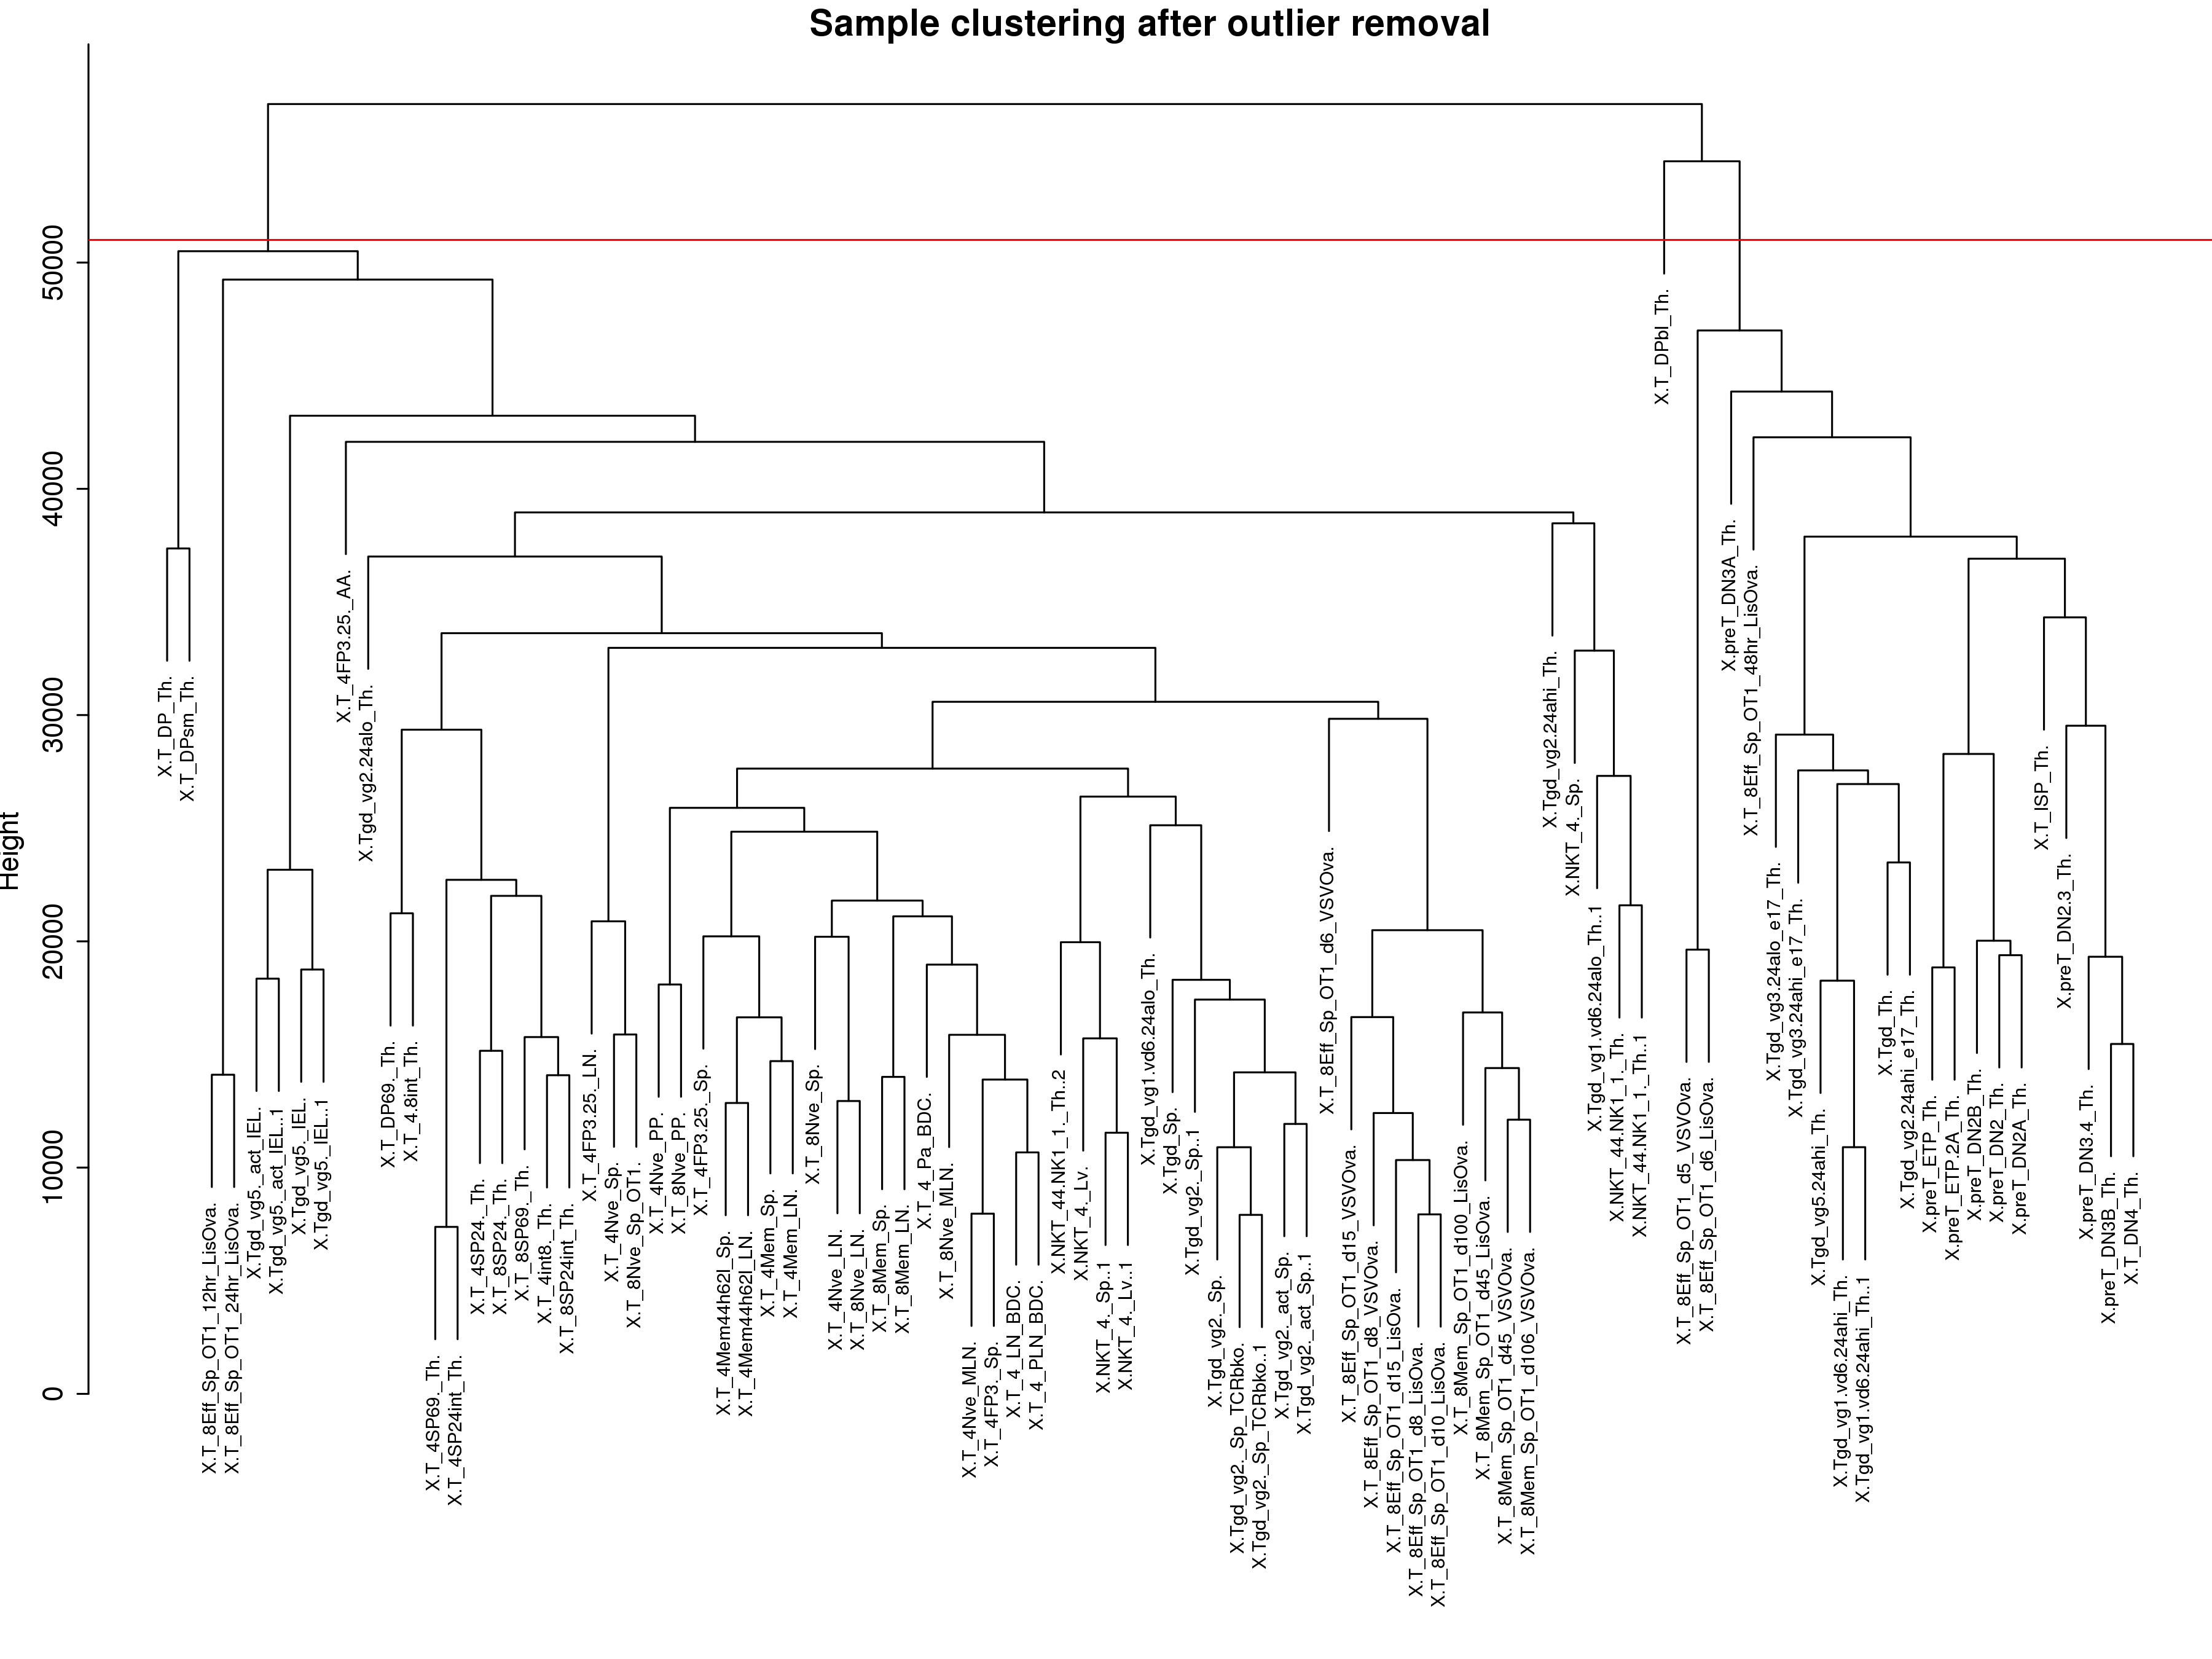
\includegraphics[width=1\textwidth]{Figures/Chapter4/WGCNA/tcell_immgen_data_sampleClustering.png}
\caption{\small{Dendrogram of ImmGen T cell dataset showing the distribution of samples following hierarchical clustering and the resulting presence of an outlier sample. The red line indicates the cut height used for the removal of this outlier. } }
    \label{fig:11}
\end{figure}

\begin{figure}[H] 
    \centering
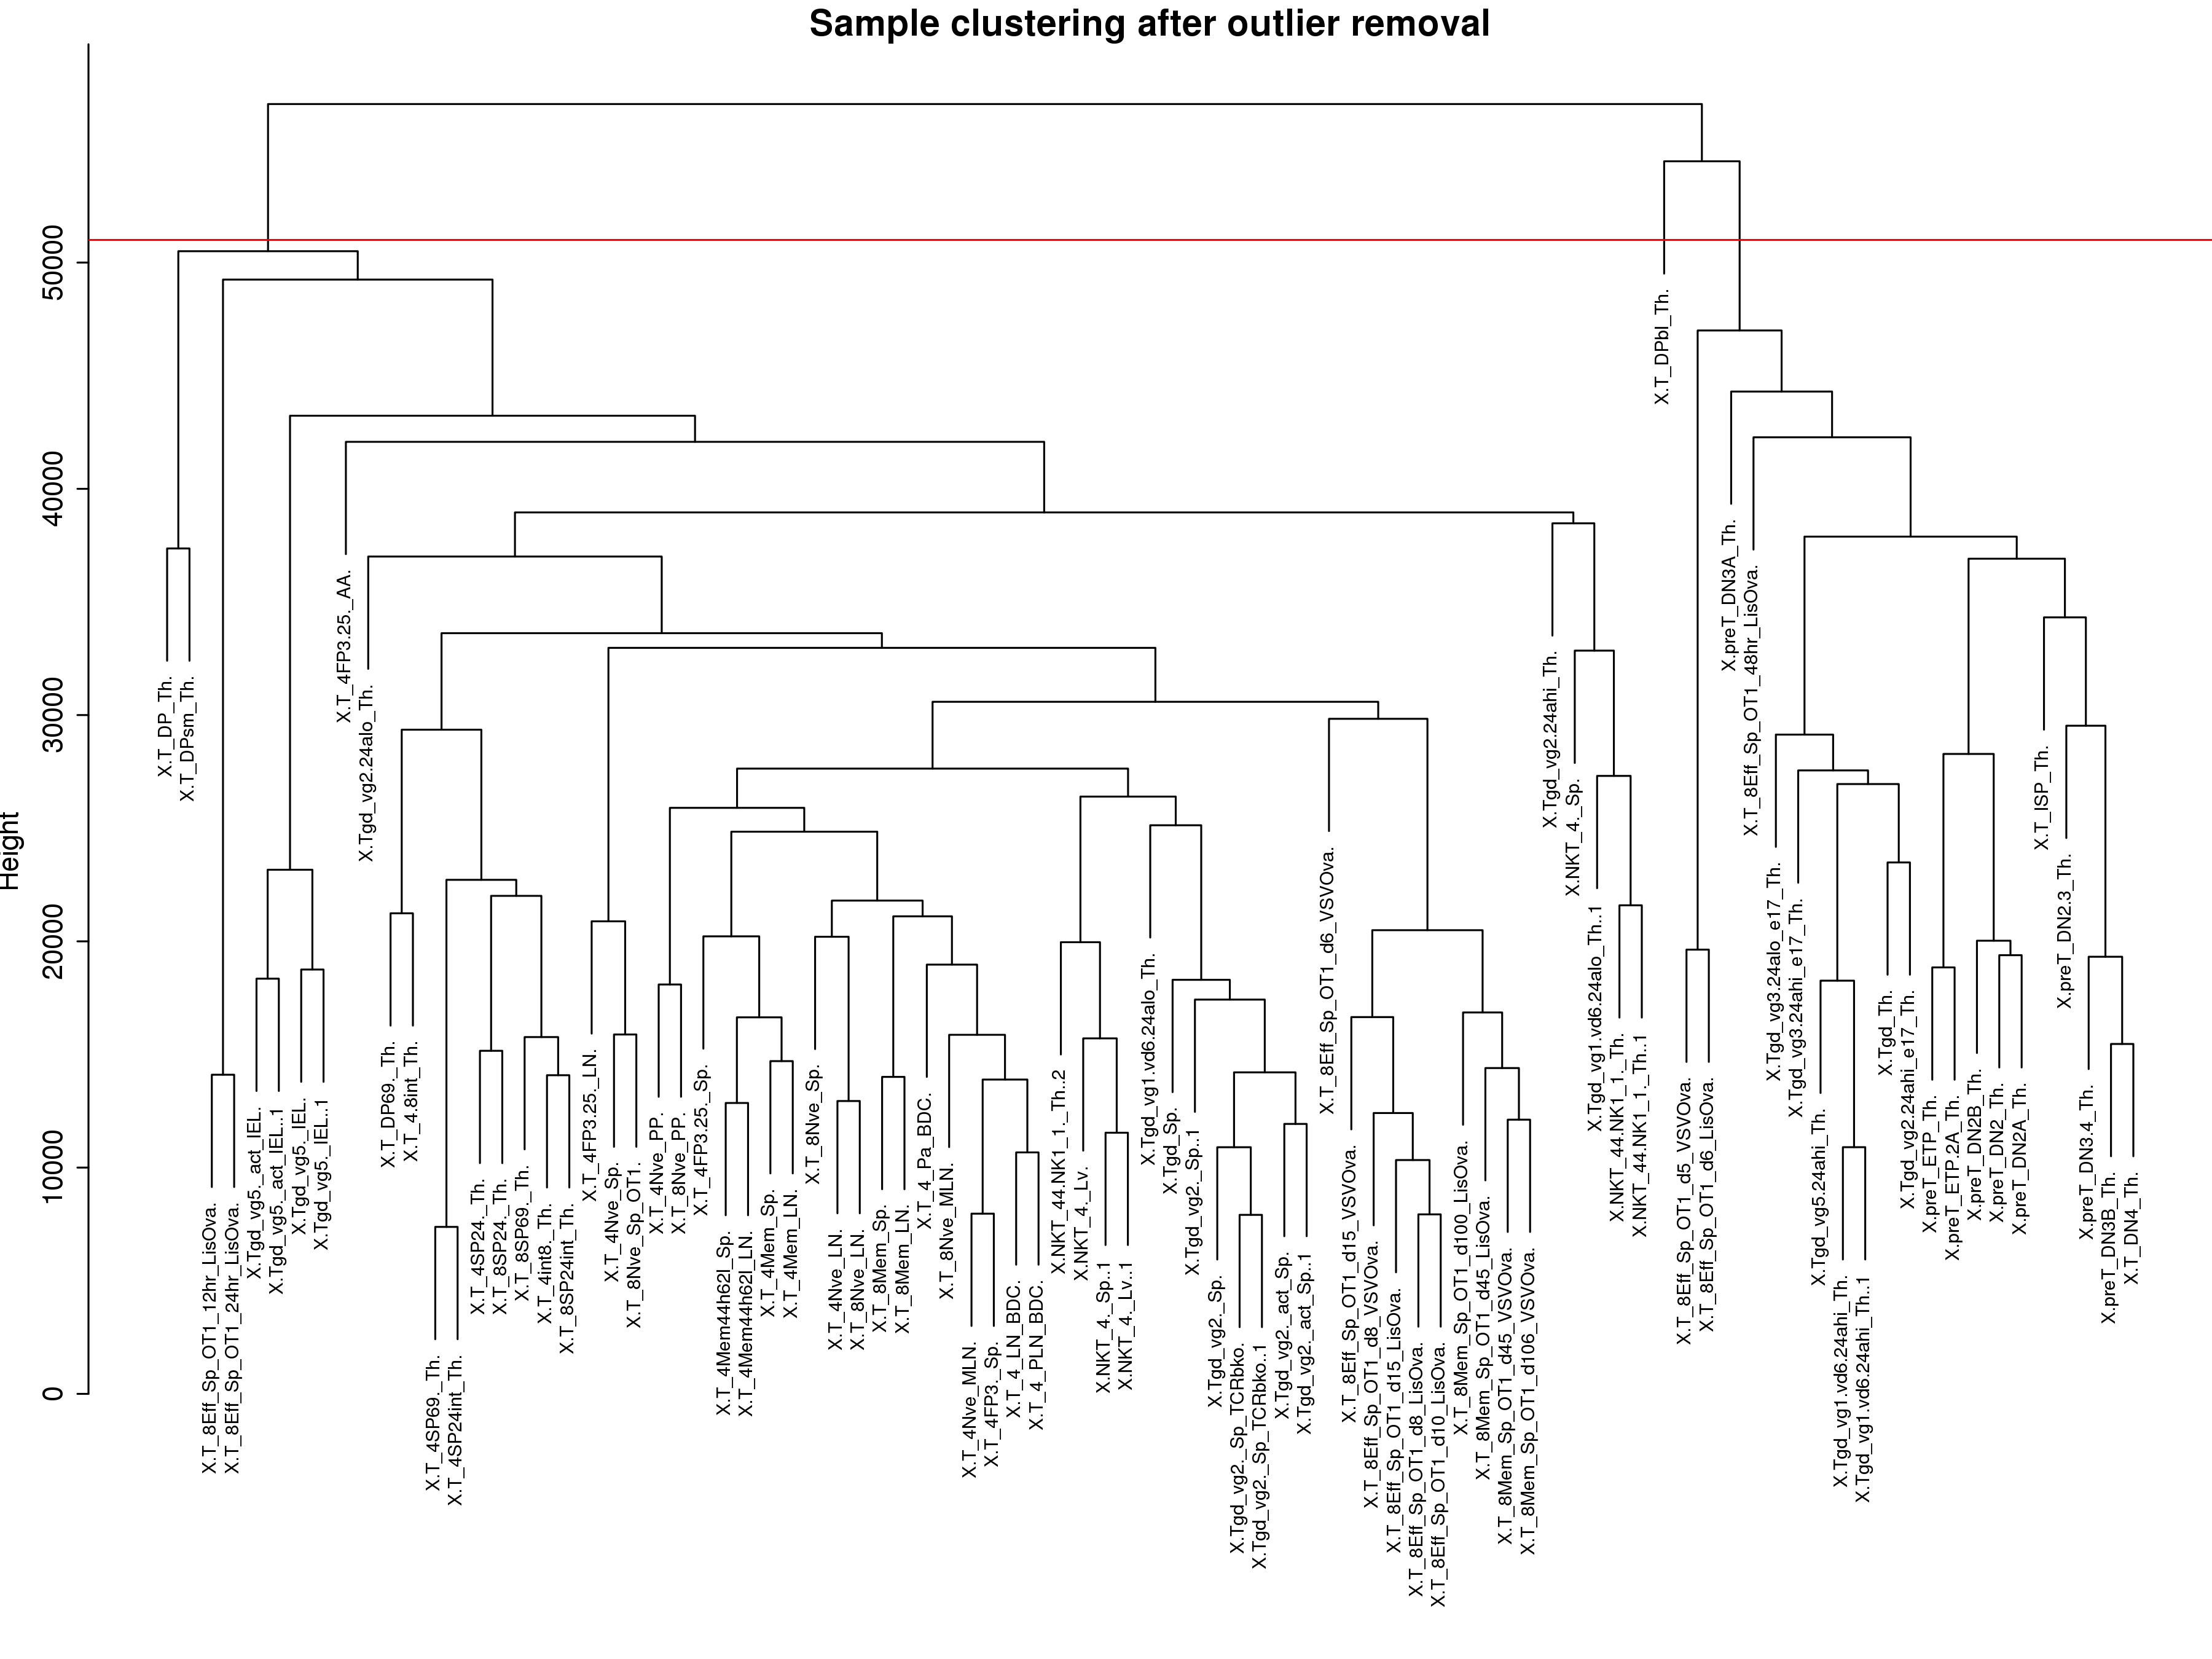
\includegraphics[width=1\textwidth]{Figures/Chapter4/WGCNA/tcell_immgen_data_sampleClustering.png}
\caption{\small{Dendrogram of ImmGen T cell dataset samples following outlier removal} }
    \label{fig:12}
\end{figure}

\begin{figure}[H] 
    \centering
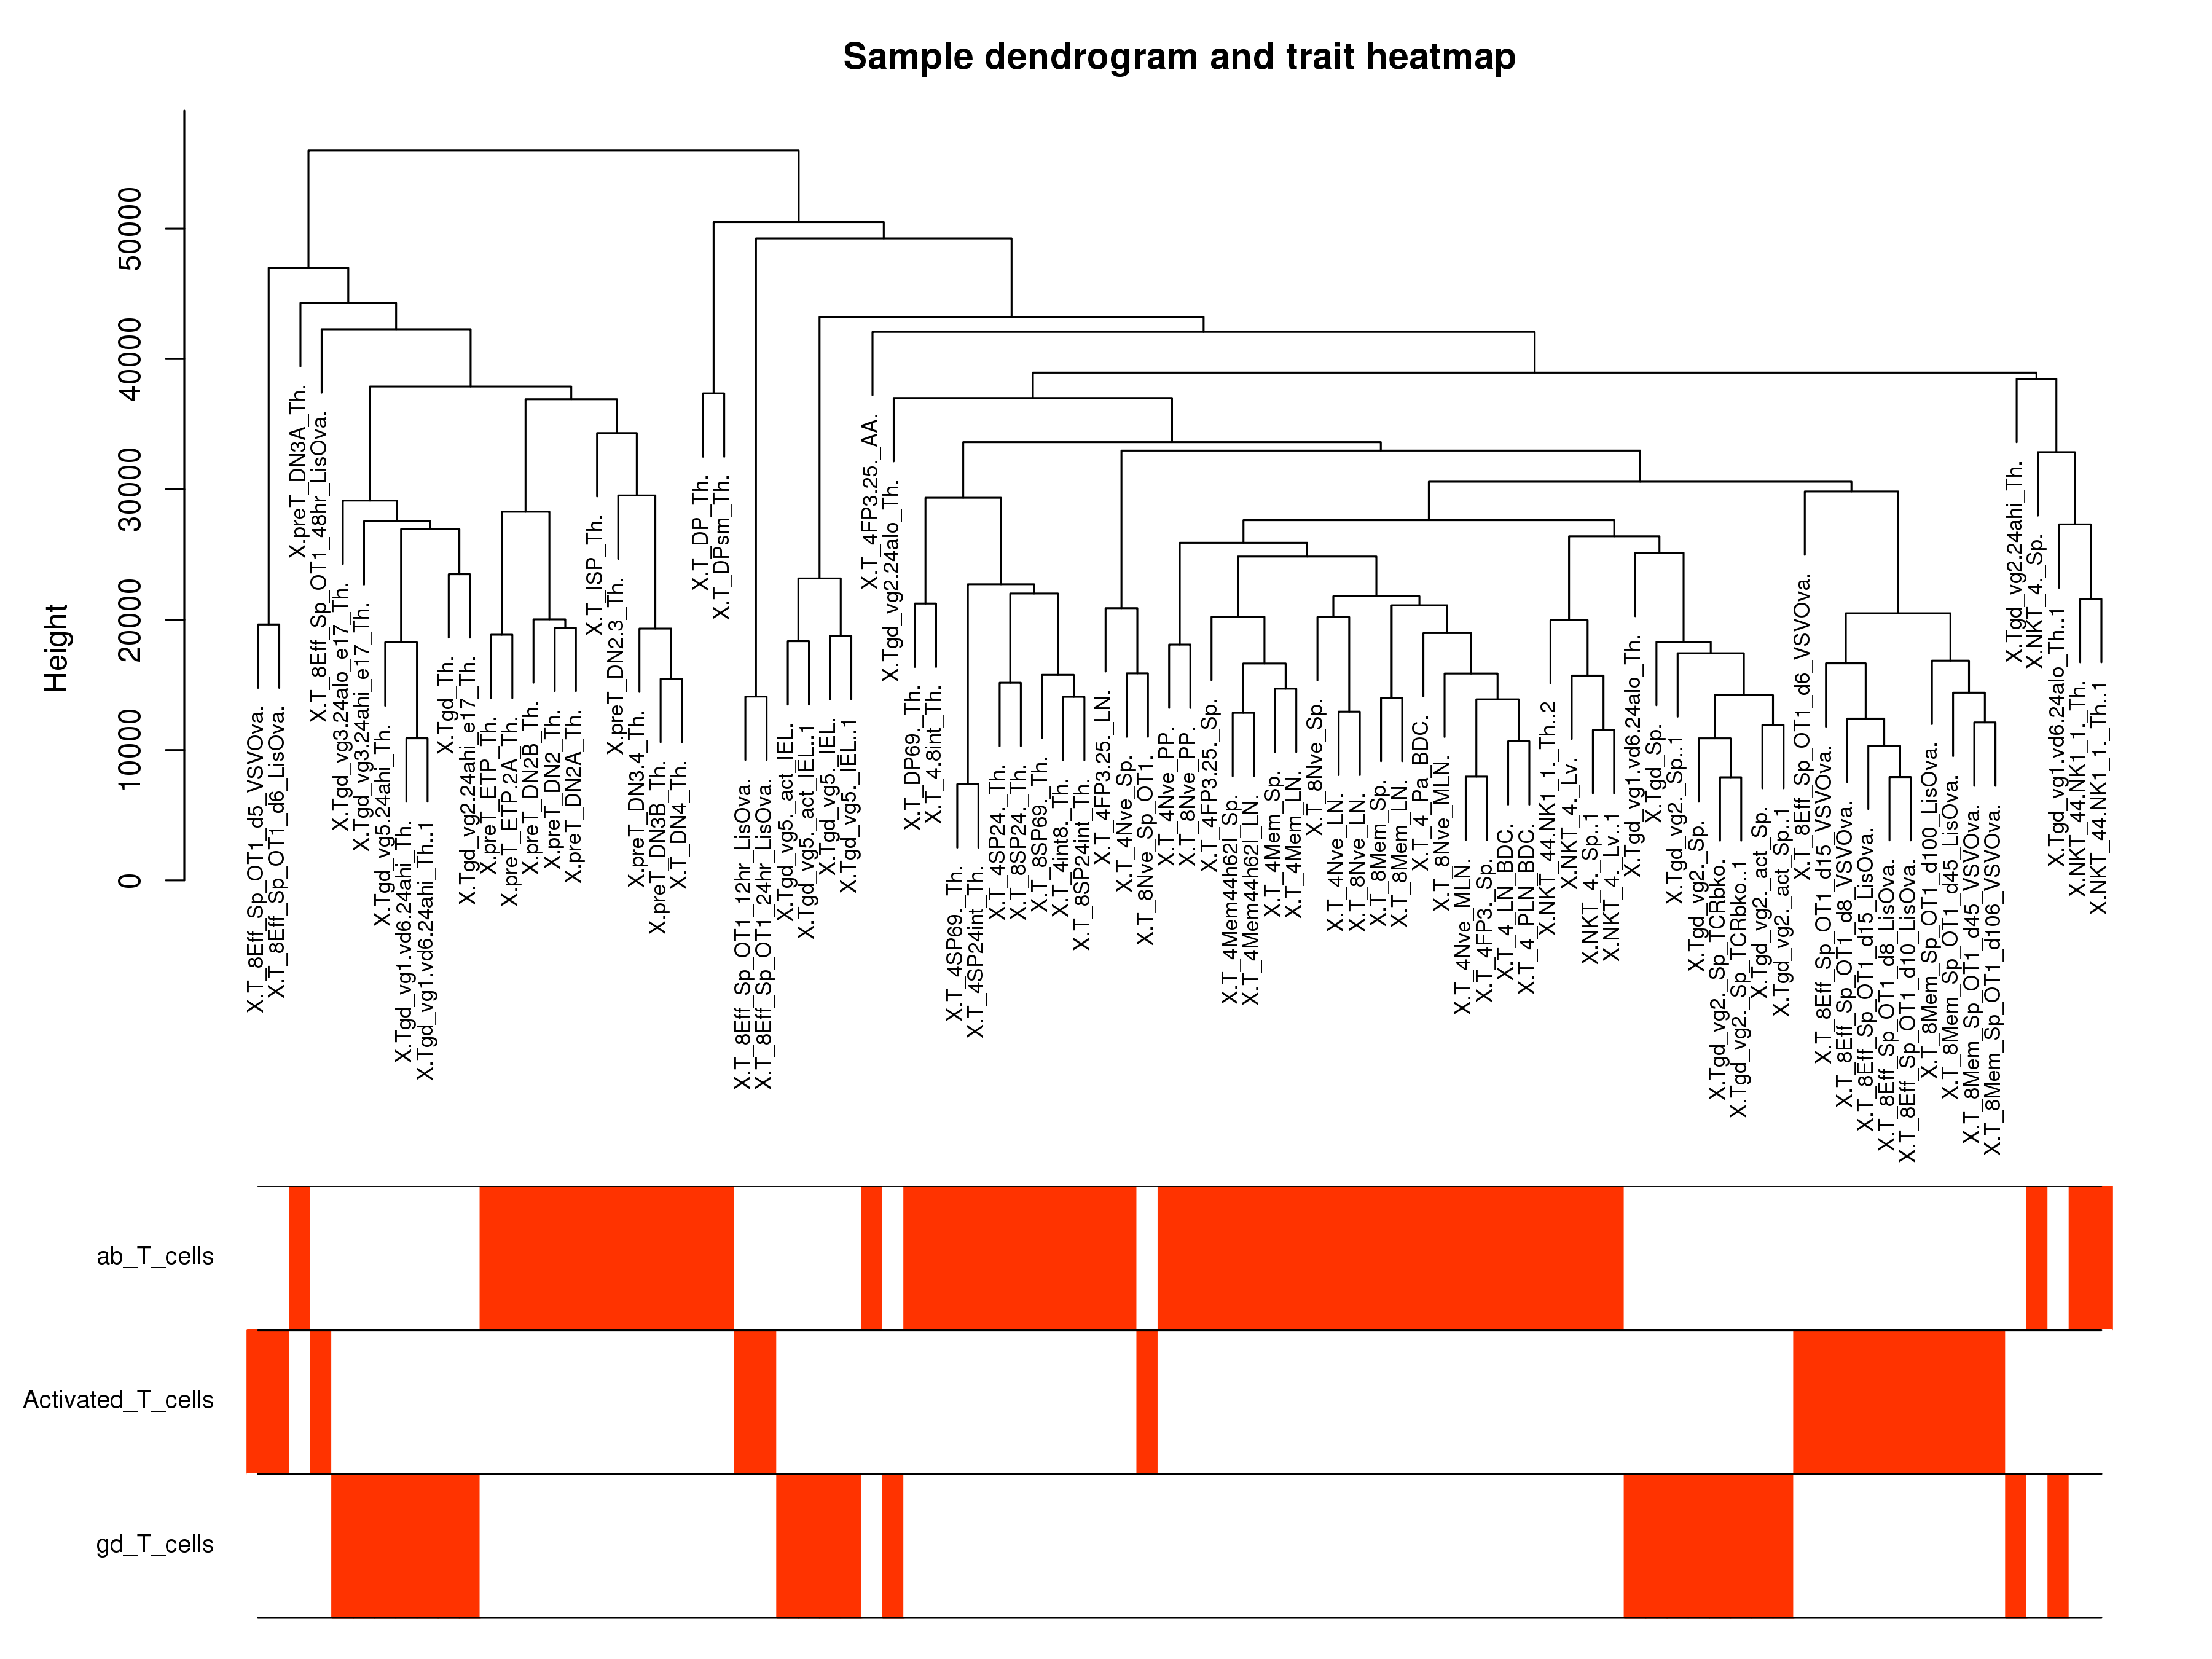
\includegraphics[width=1\textwidth]{Figures/Chapter4/WGCNA/tcell_immgen_data_dendrogram_plus_traits.png}
\caption{\small{ImmGen T cell dataset sample dendrogram with associated trait information displayed beneath.} }
    \label{fig:13}
\end{figure}

Following visual examination of the data and the necessary pre-processing steps including selection of the thresholding power (see Chapter \ref{Chapter3}) which for this dataset was selected as 39 based on modelling the scale free topology, all genes were clustered using the cutreeDynamic function of the WGCNA package. 204 gene modules were produced as a result of this gene clustering with size ranging from 1 to 6344 genes per module. Naturally, a gene module consisting of 1 or even several genes is not going to be biologically relevant and so all modules containing less than 5 genes were removed from further analysis. Similarly, it is difficult to see how a module comprising thousands of genes is likely to represent a cohesive collection of interacting genes and so the two modules whose sizes were greater than 1000 genes were also ignored in subsequent work. As mentioned in Chapter \ref{Chapter3}, WGCNA offers the option to summarise each module identified by its eigengene and Figure 4.4 shows the dendrogram of all module eigengenes produced by the gene clustering algorithm. It is clear from this plot that a number of the eigengenes are extremely closely "related" and as per the recommended analytical procedure, modules whose eigengenes were below 0.05 on the dendrogram were merged using the in built function mergeCloseModules.

\begin{figure}[H] 
    \centering
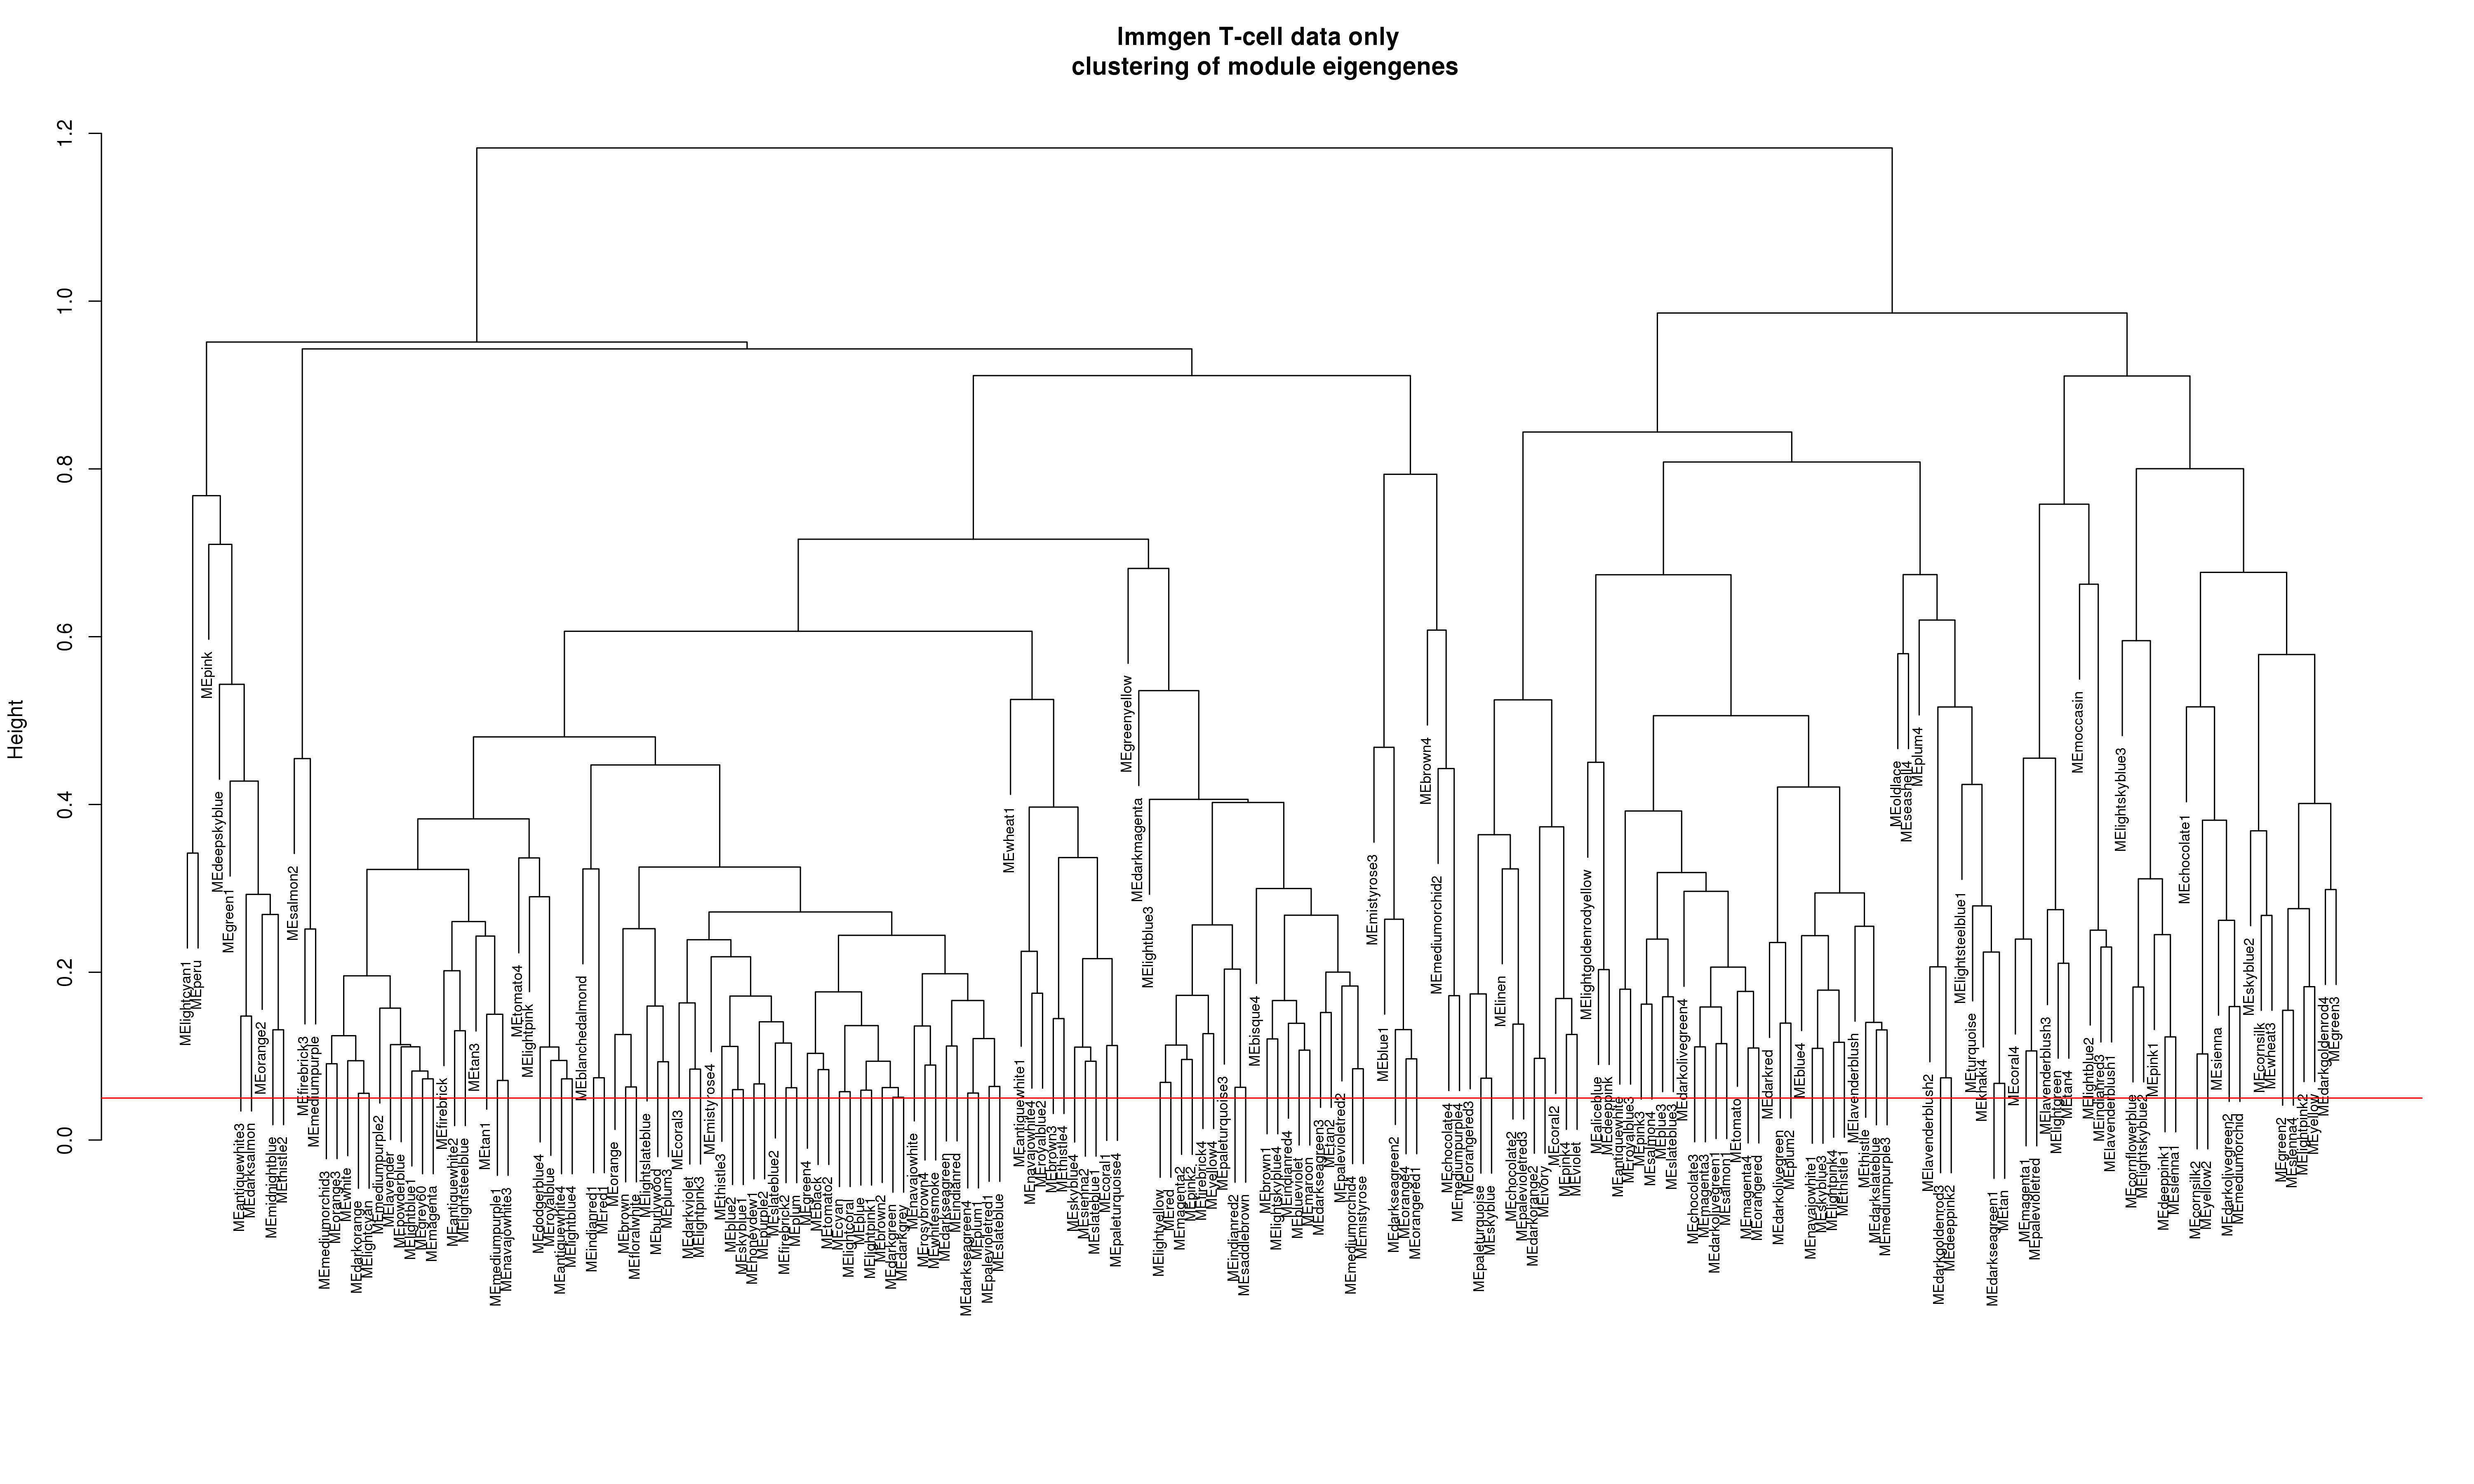
\includegraphics[width=1\textwidth]{Figures/Chapter4/WGCNA/tcell_immgen_data_module_eigengene_clustering.png}
\caption{\small{Dendrogram of the module eigengenes produced by clustering using WGCNA. The red line depicts the threshold below which modules were merged to avoid the generation of modules too small to be of biological relevance. } }
    \label{fig:14}
\end{figure}

One particularly useful feature of the WGCNA package is the ability to plot correlations between gene modules and sample traits in the form of a heatmap. This enables straightforward evaluation of whether any given module is associated with a particular trait and this is extremely useful when attempting the early stages of clustering quality evaluation and module annotation. Given the large number of modules produced in this particular analysis, it is not feasible to discuss each module individually. However, the module - trait heatmap shown in Figure 4.5 does provide a general overview of how the distribution of gene modules relates back to the T cell subtypes included in this dataset. Interestingly, the majority of correlations are very weak which would indicate that the genes they are comprised of may not all originate from a single cell type. There are a few exceptions, notably a collection of modules strongly correlated with the Activated T cell samples, but in general the results are disappointing. Without performing an in depth analysis examining each of the 204 gene modules it is difficult to determine whether poor clustering results or the splitting of tightly clustered genes across multiple modules may be the cause. 

\begin{figure}[H] 
    \centering
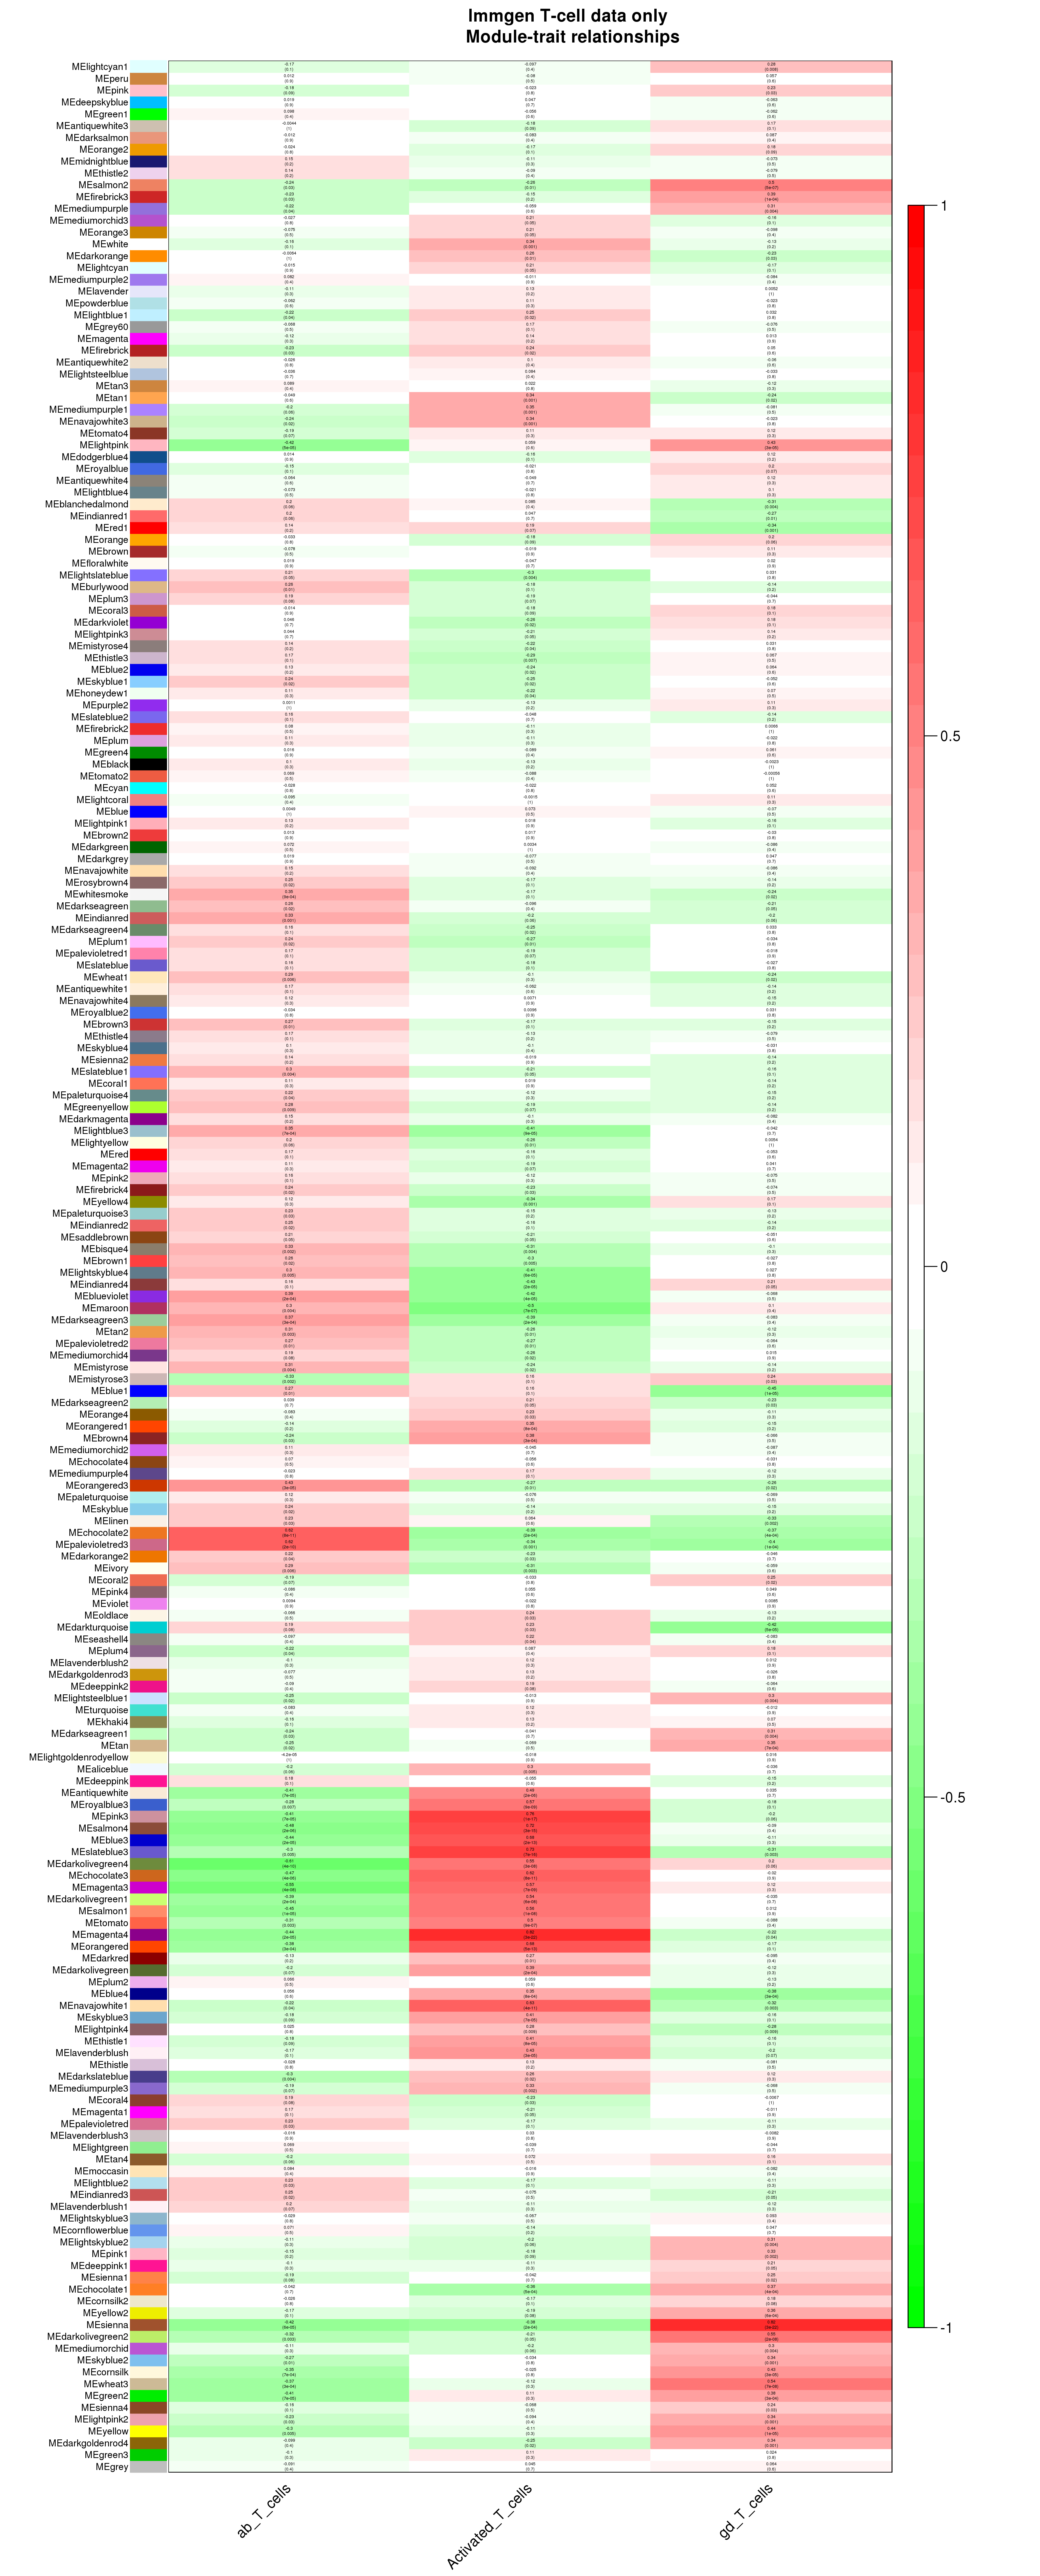
\includegraphics[width=0.58\textwidth]{Figures/Chapter4/WGCNA/tcell_immgen_data_module_trait_relationships_heatmap.png}
\caption{\small{Heatmap showing correlations between each of the WGCNA gene modules (y-axis) and the three T cell sub-populations. The colour bar to the right of the figure shows the colour coding scheme where strongly positive correlations are coloured red, strongly negative correlations are coloured green} }
    \label{fig:15}
\end{figure}

\section{Distribution of ImmGen Coarse module genes within T cell WGCNA clusters}

Table 4.1 below details how the genes within the 81 Coarse modules defined by ImmGen are distributed within the gene modules produced by reclustering the T cell data using WGCNA. The striking feature of of this table is that virtually all of the original modules defined by the ImmGen consortium have been split over multiple modules in the reclustering process. This could suggest one of two things. It may be that the observed differences in cluster solutions are simply a result of the fact that the intricacies of the algorithms used by WGCNA and PMC are quite different, WGCNA, as its name suggests, partitions data based on correlation strength while PMC does not incorporate this property of the data when clustering. Alternatively, the fact that this WGCNA analysis was performed using only T cell samples is likely to result in quite different clustering output than a more heterogeneous dataset. When the distribution of the WGCNA modules is compared to the ImmGen assignments, there do appear to be some broad similarities between the number of WGCNA modules genes of a given ImmGen Coarse module are split into and the number of Fine-grained modules reported by ImmGen. It is thus tempting to ponder whether the WGCNA modules determined in this analysis may in fact be more comparable to the ImmGen Fine modules. Whilst this could easily be quantified, we would not truly be be comparing like for like given that the ImmGen Fine modules were produced by reclustering of Course module data rather than from the expression dataset as a whole ~\autocite{Joj2013}.  

As discussed in Chapter \ref{Chapter3} only one of the Coarse modules published by ImmGen, C18, was T cell specific and was found to be comprised of genes whose functions relate to T cell activation. Given the group of WGCNA modules showing high positive correlations with the "Activated T cells" trait, we were particularly interested to determine whether there was any overlap between the genes assigned to these modules and those within Coarse module C18. The majority of genes comprising module C18 were not assigned to any of the WGCNA gene clusters analysed and hence it must be assumed that they were part of the large modules previously excluded from the WGCNA output module list. Of the C18 genes that were included in the final list of WGCNA modules, four out of a total of twelve modules showed significant correlation to the "Activated T cells" trait. These modules are: skyblue3 (\textit{p}-value = 7e\textsuperscript{-05}), thistle1 (\textit{p}-value = 8e\textsuperscript{-05}), darkslateblue (\textit{p}-value = 0.02), aliceblue (\textit{p}-value = 0.005). These modules vary in size between 16 and 56 genes which places them within the parameters of modules that are of appropriate scale to be of interest from a biological standpoint.  It is concerning however that most of the C18 genes were "lost" during WGCNA reclustering. 

\begin{landscape}
\small 
\begin{longtable}{|p{1.5cm}|p{1.25cm}|p{21cm}|}
\caption{Table detailing how genes assigned to each ImmGen Coarse module are dispersed within the modules generated by re-clustering of T cell samples with WGCNA}\\
\hline
ImmGen Coarse mod & Coarse mod size & Distribution of genes among WGCNA T cell data modules \\
\hline
1 & 334 & mediumpurple1 (6) darkred (50) salmon1 (2) darkolivegreen (22) thistle1 (7) deeppink (2) plum2 (15) lightsteelblue (4) darkolivegreen4 (2) lightpink4 (4) ivory (6) paleturquoise (2) tan4 (2) darkseagreen2 (2) skyblue (3) blue4 (4) lavenderblush1 (2) tan3 (5) brown (2) darkslateblue (2) greenyellow (5) navajowhite1 (2) white (2) yellow (2) skyblue3 (2) floralwhite (2) orangered (2) aliceblue (2) \\
2 & 229 & brown (23) floralwhite (21) orange (2) lightsteelblue (21) grey60 (14) antiquewhite2 (3) tan3 (2) black (4) darkred (2) lightskyblue4 (2) white (3) navajowhite3 (3) darkgreen (3) greenyellow (2) burlywood (2) brown1 (2) mediumpurple1 (7) lightcyan (3) lightslateblue (4) mistyrose (2) plum3 (2) tan1 (4) blue (4) darkorange (4) orangered3 (2) \\
3 & 344 & magenta (24) floralwhite (6) lightcoral (51) darkgrey (16) cyan (12) orangered1 (2) dodgerblue4 (4) royalblue (6) lightsteelblue (6) blue (16) brown2 (6) honeydew1 (2) lightpink3 (6) lightblue1 (7) black (4) grey60 (7) darkgreen (3) lightblue4 (5) darkviolet (2) antiquewhite2 (4) lightpink (5) indianred4 (2) brown (3) firebrick4 (2) antiquewhite4 (6) lightcyan (3) white (5) thistle3 (2) darkorange (2) \\
4 & 118 & skyblue4 (10) sienna2 (4) brown3 (3) slateblue1 (2) thistle4 (9) coral1 (4) lightblue1 (3) blue (3) lightcoral (4) dodgerblue4 (2) \\
5 & 313 & grey60 (27) darkorange (30) royalblue (5) orange3 (3) lightcyan (47) mediumpurple2 (3) cyan (3) blue (21) rosybrown4 (2) greenyellow (6) lightpink1 (9) darkseagreen3 (2) mediumorchid3 (4) floralwhite (13) bisque4 (5) lightsteelblue (4) black (5) darkgreen (6) white (7) lightcoral (3) mistyrose (2) magenta (4) brown (6) maroon (3) saddlebrown (2) indianred1 (3) lightblue1 (3) thistle3 (2) lightblue4 (2) \\
6 & 111 & lightcoral (5) magenta (13) lightcyan (6) grey60 (7) blue (14) antiquewhite4 (2) cyan (7) floralwhite (2) darkgrey (4) darkgreen (3) brown2 (2) mediumpurple2 (3) lightpink1 (2) slateblue (2) lightblue1 (3) brown (2) lightblue4 (3) plum (2) \\
7 & 30 & black (2) floralwhite (5) darkgreen (7) lightpink1 (3) \\
8 & 23 & floralwhite (3) antiquewhite4 (4) magenta (3) brown (2) \\
9 & 15 & blue (3) lightcyan (3) \\
10 & 14 & lightpink1 (3) blue (2) lightcyan (2) \\
11 & 153 & brown (91) orange (22) black (2) floralwhite (3) \\
12 & 46 & floralwhite (15) black (8) brown (14) \\
13 & 101 & honeydew1 (2) black (8) blue (8) floralwhite (12) lavender (3) maroon (5) cyan (2) darkgreen (3) plum3 (3) yellow4 (2) brown (2) plum1 (2) greenyellow (3) \\
14 & 73 & brown (34) floralwhite (21) blue (2) black (2) \\
15 & 38 & floralwhite (20) black (9) brown (3) \\
16 & 363 & blue (3) grey60 (3) thistle1 (3) violet (11) thistle (9) orangered3 (9) navajowhite1 (3) skyblue (18) darkslateblue (5) paleturquoise (10) darkorange2 (4) darkolivegreen4 (2) pink4 (2) coral2 (4) skyblue3 (11) black (2) mediumpurple3 (4) ivory (7) lightcyan (5) lightcoral (2) greenyellow (4) salmon2 (2) tomato (2) darkolivegreen1 (2) pink3 (2) palevioletred2 (2) lightpink1 (2) linen (3) white (2) yellow (2) salmon1 (2) palevioletred3 (3) magenta (2) \\
17 & 201 & thistle1 (15) lightpink2 (4) salmon4 (4) navajowhite1 (5) thistle (2) darkolivegreen (2) darkseagreen3 (2) lavenderblush (2) skyblue3 (7) brown (3) lightpink4 (5) darkslateblue (5) skyblue (4) coral2 (2) lightgreen (2) paleturquoise (3) mediumpurple3 (4) pink4 (4) violet (2) royalblue (2) saddlebrown (2) floralwhite (2) yellow (2) \\
18 & 146 & linen (3) orangered3 (8) skyblue3 (2) skyblue (4) darkgoldenrod4 (2) greenyellow (2) thistle1 (2) yellow (7) lightpink2 (5) darkslateblue (3) aliceblue (2) paleturquoise (2) \\
19 & 125 & darkmagenta (2) darkolivegreen1 (3) pink3 (3) yellow (14) sienna4 (3) brown4 (5) magenta4 (8) tomato (2) darkolivegreen4 (8) deeppink (4) chocolate3 (3) aliceblue (2) skyblue3 (2) midnightblue (2) salmon4 (2) skyblue2 (2) royalblue3 (3) orangered (5) wheat3 (2) lightskyblue3 (4) \\
20 & 54 & \\
21 & 82 & orangered1 (5) blue1 (2) darkolivegreen (3) darkseagreen2 (3) \\
22 & 39 & brown (4) darkred (5) darkseagreen2 (2) firebrick (2) lightsteelblue (2) tan3 (2) \\
23 & 54 & lightcoral (2) honeydew1 (2) lightsteelblue (2) darkgrey (2) floralwhite (6) blue (6) royalblue (3) cyan (3) grey60 (2) lightblue4 (3) \\
24 & 486 & blueviolet (2) lightgreen (10) midnightblue (13) magenta (5) red (21) lightyellow (9) saddlebrown (7) pink (27) thistle2 (4) darkolivegreen2 (3) coral3 (4) lightcoral (4) lightcyan (4) plum (6) yellow (24) mediumorchid4 (3) green3 (3) darkolivegreen4 (2) antiquewhite3 (2) lightsteelblue1 (4) darkmagenta (4) pink2 (3) honeydew1 (2) lightcyan1 (3) greenyellow (5) lavenderblush3 (3) coral4 (5) blue3 (2) tan4 (3) darkseagreen3 (2) mediumpurple (4) lightblue1 (3) yellow4 (3) floralwhite (2) brown4 (2) blue2 (3) sienna4 (2) blue (4) mediumorchid (3) thistle3 (3) \\
25 & 438 & pink (47) red (20) yellow (16) orangered (2) midnightblue (25) magenta4 (2) floralwhite (5) honeydew1 (2) darkolivegreen2 (6) lightskyblue3 (2) mediumorchid (10) blue (5) salmon4 (7) lightyellow (11) magenta1 (4) thistle2 (10) brown4 (3) skyblue2 (2) darkmagenta (2) indianred3 (2) palevioletred3 (2) tan4 (2) lightblue3 (2) orangered3 (2) royalblue3 (4) thistle1 (2) magenta2 (2) magenta3 (2) darkolivegreen4 (4) lightcyan1 (2) palevioletred (2) lightcoral (2) lightgreen (4) grey60 (2) \\
26 & 247 & lightcoral (2) red (6) thistle2 (3) lightcyan1 (3) yellow (6) lightgreen (4) lightyellow (8) mediumorchid (4) pink (3) saddlebrown (2) yellow4 (2) black (2) darkmagenta (2) maroon (2) green3 (2) \\
27 & 72 & plum3 (2) blue (2) greenyellow (2) brown4 (2) \\
28 & 55 & thistle2 (2) pink (3) red (4) midnightblue (3) lightsteelblue1 (2) brown4 (2) yellow (3) \\
29 & 37 & lightgreen (2) red (6) midnightblue (2) yellow (3) magenta1 (2) orange2 (2) antiquewhite3 (2) \\
30 & 76 & pink (16) red (3) darksalmon (2) darkgreen (2) midnightblue (2) lightgreen (3) thistle2 (2) \\
31 & 40 & pink (13) yellow (2) \\
32 & 101 & lightgreen (10) coral4 (10) yellow (5) magenta1 (2) brown4 (3) palevioletred (3) aliceblue (2) \\
33 & 147 & blueviolet (2) skyblue3 (2) greenyellow (3) plum4 (6) lightcyan1 (2) darkmagenta (2) red (4) lightgreen (3) mediumorchid (2) midnightblue (3) tan2 (2) thistle2 (3) black (2) pink (2) indianred4 (3) mediumorchid4 (3) \\
34 & 117 & skyblue3 (4) lavenderblush1 (3) yellow (5) thistle (4) mediumpurple3 (13) darkslateblue (2) chocolate4 (2) salmon1 (2) lightcoral (2) lightpink4 (2) navajowhite1 (2) \\
35 & 268 & deepskyblue (2) darkmagenta (2) lavenderblush3 (5) lightgreen (3) mistyrose (2) lightcyan1 (3) yellow (2) \\
36 & 202 & pink (2) brown4 (2) skyblue2 (2) yellow (3) darkmagenta (2) firebrick3 (2) lightcyan1 (2) deeppink1 (2) \\
37 & 41 & \\
38 & 42 & \\
39 & 45 & \\
40 & 67 & firebrick4 (2) thistle2 (4) yellow4 (2) midnightblue (5) lightyellow (3) red (3) lightgreen (2) lightskyblue3 (2) \\
41 & 54 & midnightblue (2) \\
42 & 53 & thistle2 (3) midnightblue (5) lightyellow (6) blue (4) red (7) honeydew1 (2) magenta2 (2) skyblue1 (2) \\
43 & 46 & lightyellow (2) midnightblue (4) red (6) indianred2 (2) lightblue2 (2) \\
44 & 118 & darkgrey (2) blue2 (2) skyblue2 (2) blue (2) yellow (3) firebrick2 (2) greenyellow (3) yellow4 (2) darkolivegreen2 (3) midnightblue (2) red (12) mediumorchid (3) black (2) firebrick3 (2) darkviolet (3) cyan (4) lightpink3 (2) lightcoral (2) thistle3 (3) \\
45 & 315 & maroon (2) floralwhite (5) salmon1 (2) slateblue3 (2) yellow (13) lightskyblue2 (3) lightsteelblue (4) lightgreen (4) navajowhite3 (2) chocolate3 (3) antiquewhite (4) darkolivegreen2 (2) darkolivegreen (6) royalblue3 (3) brown4 (2) midnightblue (2) navajowhite1 (3) salmon4 (3) magenta3 (6) darkolivegreen4 (5) darkolivegreen1 (3) pink3 (4) mediumpurple3 (3) red (4) brown (2) plum1 (2) darkred (2) tan4 (3) deeppink (2) mistyrose3 (2) aliceblue (2) thistle (2) orangered (3) \\
46 & 155 & yellow (5) lightcoral (14) coral1 (2) magenta (6) blue (4) cyan (7) darkgrey (6) black (2) royalblue (4) lightpink3 (3) darkgreen (3) lightcyan (2) cornsilk (2) brown (2) \\
47 & 134 & red (8) maroon (2) darkgreen (4) lightcyan (3) blue2 (5) floralwhite (5) indianred4 (11) blueviolet (5) firebrick4 (6) midnightblue (2) lavender (2) blue (4) magenta2 (4) black (8) lightyellow (6) honeydew1 (5) yellow4 (3) brown1 (2) greenyellow (2) grey60 (2) plum3 (2) indianred2 (2) \\
48 & 134 & darkslateblue (2) navajowhite1 (2) lightcyan1 (2) skyblue (5) greenyellow (4) palevioletred2 (2) floralwhite (2) darkolivegreen2 (2) yellow (5) paleturquoise (2) salmon4 (2) \\
49 & 108 & mistyrose4 (3) lightyellow (2) floralwhite (3) royalblue (5) thistle3 (2) black (3) red (3) lightsteelblue (3) honeydew1 (3) grey60 (3) brown (2) cyan (2) antiquewhite2 (2) lightcoral (3) \\
50 & 91 & plum1 (5) skyblue1 (2) saddlebrown (2) whitesmoke (2) darkviolet (2) midnightblue (2) floralwhite (3) blueviolet (5) red (5) blue (2) indianred4 (2) black (4) \\
51 & 51 & darkolivegreen (6) plum2 (4) darkred (9) mediumpurple1 (3) \\
52 & 149 & chocolate4 (11) mediumpurple4 (18) yellow (4) skyblue3 (6) skyblue (6) thistle (3) paleturquoise (9) brown4 (2) coral2 (3) navajowhite1 (2) mediumorchid2 (2) \\
53 & 97 & lightsteelblue1 (3) coral2 (3) yellow (7) paleturquoise (2) sienna4 (2) lightcyan1 (2) skyblue3 (2) salmon4 (2) lightgreen (2) mediumpurple3 (2) magenta3 (2) \\
54 & 38 & darkslateblue (4) skyblue3 (2) \\
55 & 26 & floralwhite (5) lightsteelblue (3) brown (4) \\
56 & 71 & cornflowerblue (6) salmon2 (12) lightcyan1 (4) pink1 (4) mediumpurple (2) lightyellow (2) deeppink (2) firebrick3 (2) \\
57 & 64 & greenyellow (17) palevioletred2 (7) chocolate1 (2) mistyrose (2) lightskyblue4 (2) tan2 (2) \\
58 & 55 & deeppink1 (2) pink (4) lightcyan1 (2) \\
59 & 15 & lightpink4 (3) \\
60 & 19 & firebrick3 (5) pink (2) \\
61 & 45 & darkgoldenrod4 (2) indianred3 (2) paleturquoise (2) yellow (2) skyblue3 (2) \\
62 & 62 & magenta3 (2) greenyellow (2) yellow (8) \\
63 & 37 & blue (2) \\
64 & 26 & yellow (2) darkslateblue (4) green3 (2) blue3 (2) \\
65 & 37 & yellow (25) \\
66 & 21 & lightsteelblue1 (2) \\
67 & 19 & paleturquoise (2) lightpink4 (2) skyblue3 (4) \\
68 & 14 & yellow2 (9) cornsilk2 (2) \\
69 & 22 & \\
70 & 13 & lavenderblush1 (2) \\
71 & 19 & yellow (2) saddlebrown (2) sienna4 (2) \\
72 & 13 & \\
73 & 12 & \\
74 & 15 & \\
75 & 12 & \\
76 & 15 & salmon2 (3) \\
77 & 11 & chocolate1 (2) \\
78 & 18 & greenyellow (2) \\
79 & 7 & \\
80 & 56 & yellow (2) pink (2) palevioletred1 (2) \\
81 & 211 & lightcyan (2) greenyellow (3) lightgreen (3) floralwhite (3) yellow (8) lightslateblue (2) pink (6) indianred3 (2) orange (2) moccasin (2) blue (2) lavenderblush3 (3) magenta4 (3) grey60 (2) lightsteelblue1 (3) brown (4) orange4 (2) \\
\hline
\end{longtable}
\end{landscape}

\section{Agglomerative Hierarchical clustering (Hclust)}

To provide a contrasting approach to the reclustering of the ImmGen T cell dataset with WGCNA, a hierarchical clustering algorithm was applied. Details of this methodology are provided in Chapter \ref{3}, but in summary the dataset was put through a two stage analysis whereby a correlation matrix was initially created using the "Person" method to calculate correlations between the expression profiles of all genes, before this correlation matrix was partitioned into clusters using Ward's method to measure the dissimilarity between observations. The output of this initial clustering was the dendrogram depicted in Figure 4.6. In contrast to WGCNA and other clustering algorithms, hierarchical clustering of a dataset is dependent upon manual specification of the desired number of clusters into which data should be split. To make this decision it is naturally necessary to make a visual inspection of the data and when analysing a significant number of genes, as was the case here, this can be problematic.  As Figure 4.6 and 4.7 show, even after two iterations it was not possible to determine the appropriate number of clusters between which to split the data and so the decision was made to iteratively partition the data into two clusters until such time as a greater number of separate, well-defined clusters were visible.

This technique is very time consuming and initially memory intensive, but it does afford the dubious advantage of being in complete control of the clustering process. Indeed, such a technique does hold an inherently higher risk of falling victim of human error but it is nevertheless still a popular choice for gene clustering analysis. One major challenge when performing hierarchical clustering on a dataset is that there is often no clear indication of when to stop partitioning the data and this could potentially result in meaningful gene clusters being either lost within a larger group, or perhaps more detrimentally being split between multiple modules. Both outcomes have the potential render the whole clustering process as effectively pointless. Following the careful and systematic clustering of the ImmGen T cell dataset, 443 modules were defined. This number is clearly much greater than in the previous analysis using WGCNA and indeed is almost incomparable to the original number published by ImmGen, which it should not be forgotten, included all immune cell types. Although the quality of the hierarchical clustering solution should naturally be assessed using measures outlined in Chapter \ref{Chapter1}, this drastic increase in the number of modules generated may suggest that the data may have been "over-clustered" resulting in many small gene modules which in reality are most likely to represent sub-modules. This is supported by the fact that although the modules produced ranged in size between 4 and 419 genes, over three quarters contained less than 100 genes and around half less than 50. Again however, it is important to stress that is a purely quantitative assessment and the qualitative analysis of these modules is still to be completed.  


\begin{figure}[H] 
    \centering
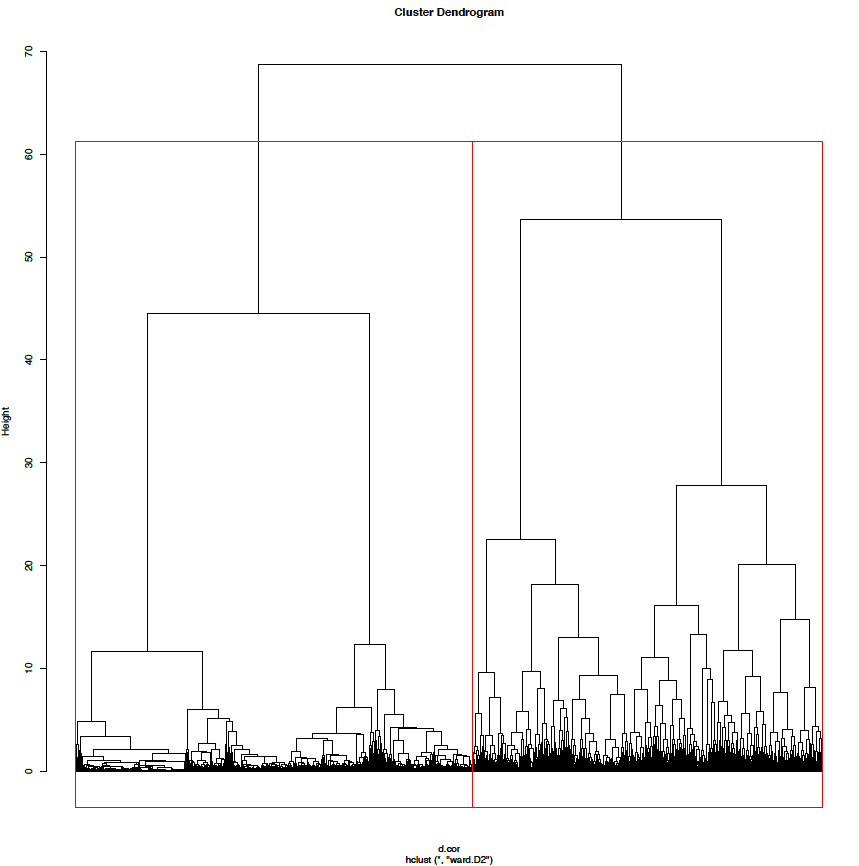
\includegraphics[width=0.9\textwidth]{Figures/Chapter4/hclust/immgen_tcell_only_hclust.png}
\caption{\small{Initial dendrogram resulting from hierarchical clustering of the ImmGen T cell dataset. Red borders separate the two clusters which will from the output of the first iteration (Clusters 1 and 2) } }
   \label{fig:16}
\end{figure}


\begin{figure}[H] 
    \centering
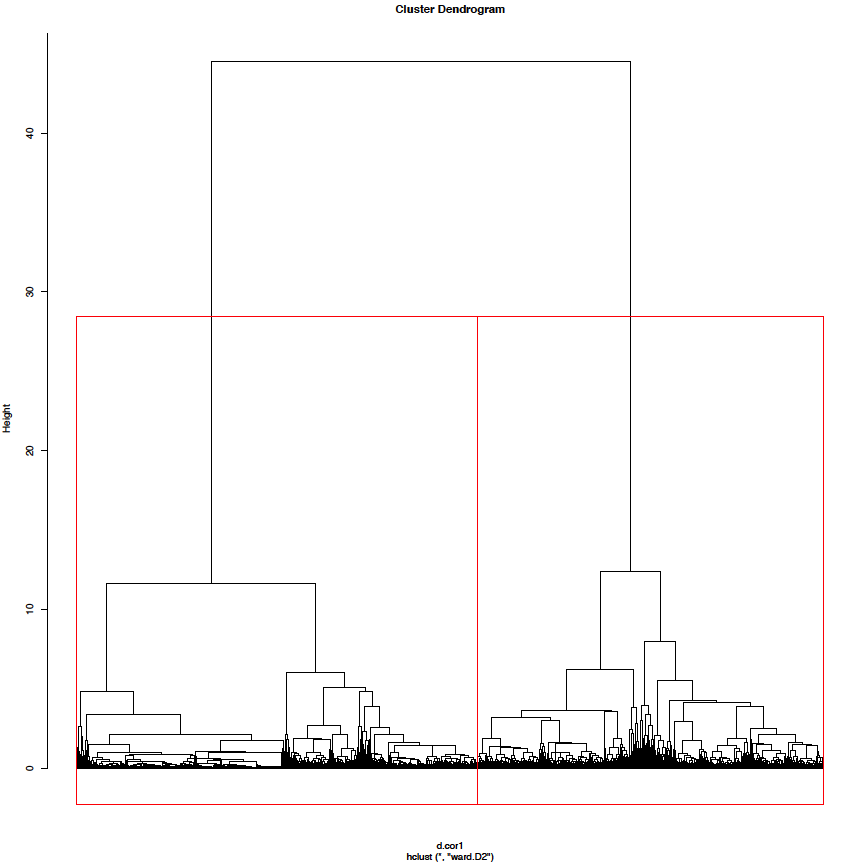
\includegraphics[width=0.9\textwidth]{Figures/Chapter4/hclust/immgen_tcell_only_hclust_CLUSTER1.png}
\caption{\small{Dendrogram depicting the result of hierarchical clustering of Cluster 1. Again, the data is partitioned into two clusters due to a lack of more detailed visual information regarding cluster separation. } }
\label{fig:17}
\end{figure}



\section{Distribution of ImmGen Coarse module genes within Tcell Hclust clusters}

Given the large number of gene modules produced by hierarchical clustering, it is perhaps unsurprising that when the distribution of genes among these clusters is compared to the ImmGen Coarse modules, the results are somewhat difficult to interpret from a biological perspective. Indeed, as can be seen from Table 4.2, when genes from a given ImmGen Coarse module are matched to a hierarchical clustering module, the overlap only extends to several genes at most. This is concerning as given that the ImmGen assignments all show at least a degree of cohesion in terms of functional annotation, the distribution of hierarchical clustering modules suggests that these properties have been lost during module partitioning. As both WGCNA and this form of hierarchical clustering separate observations based on correlations it would be interesting to directly compare their results to see how similar or otherwise the module assignments are.  

\begin{landscape}
\small 
\begin{longtable}{|p{1.5cm}|p{1.25cm}|p{21cm}|}
\caption{Table detailing how genes assigned to each ImmGen Coarse module are dispersed within the modules generated by re-clustering of T cell samples with Hclust}\\
\hline
ImmGen Coarse mod & Coarse mod size & Distribution of genes among Hclust T cell data modules \\
\hline
1 & 334 & 297 (2) 300 (2) 325 (2) 347 (2) 349 (3) 353 (2) 354 (3) 361 (3) 362 (6) 365 (4) 380 (11) 381 (4) 390 (27) 391 (7) 392 (5) 393 (33) 395 (4) 398 (8) 399 (9) 403 (2) 407 (3) 408 (3) 412 (2) 419 (22) 420 (8) 422 (17) 429 (3) 431 (2) 438 (23) 439 (12) 440 (6) \\
2 & 229 & 266 (2) 269 (2) 270 (10) 276 (2) 278 (2) 287 (2) 292 (3) 295 (2) 297 (4) 298 (4) 300 (3) 303 (14) 308 (2) 325 (8) 326 (5) 327 (3) 336 (2) 347 (3) 348 (6) 349 (12) 350 (6) 353 (4) 354 (5) 362 (4) 364 (2) 368 (2) 374 (4) 382 (2) 390 (6) 392 (5) 393 (7) 394 (2) 395 (3) 398 (4) 399 (2) 400 (3) 419 (8) 422 (3) 430 (2) \\
3 & 344 & 4 (2) 255 (2) 266 (4) 268 (8) 269 (4) 270 (3) 272 (9) 274 (4) 275 (12) 278 (4) 284 (4) 285 (2) 288 (5) 290 (4) 297 (23) 298 (15) 302 (4) 303 (17) 308 (2) 310 (2) 312 (8) 319 (5) 320 (7) 324 (2) 325 (2) 327 (7) 336 (2) 347 (5) 348 (3) 349 (21) 350 (2) 353 (24) 354 (15) 355 (3) 361 (2) 368 (2) 374 (2) 382 (3) 390 (6) 393 (4) 398 (3) 400 (3) 412 (2) 419 (4) 439 (2) \\
4 & 118 & 275 (2) 280 (2) 297 (2) 307 (2) 323 (12) 324 (5) 325 (2) 326 (3) 327 (2) 335 (6) 336 (5) 339 (9) 340 (2) 347 (2) 350 (5) 354 (2) \\
5 & 313 & 266 (3) 267 (6) 268 (2) 269 (2) 270 (3) 271 (2) 273 (13) 277 (3) 278 (2) 280 (4) 284 (5) 285 (6) 287 (3) 288 (2) 297 (8) 298 (31) 300 (5) 302 (2) 303 (7) 308 (18) 310 (2) 319 (2) 320 (7) 321 (5) 322 (14) 324 (4) 325 (4) 326 (2) 327 (4) 336 (3) 347 (2) 348 (2) 349 (9) 350 (2) 353 (19) 354 (13) 355 (2) 364 (2) 375 (2) 383 (2) 386 (2) 390 (5) 392 (3) 393 (3) 394 (3) 419 (2) 430 (2) 431 (3) 439 (4) 440 (2) \\
6 & 111 & 268 (3) 272 (2) 273 (3) 275 (5) 284 (2) 285 (3) 288 (3) 298 (9) 303 (4) 308 (4) 312 (6) 320 (5) 322 (3) 325 (2) 347 (2) 348 (3) 349 (2) 353 (16) 354 (7) \\
7 & 30 & 285 (2) 303 (2) 310 (2) 319 (4) 325 (4) 327 (5) \\
8 & 23 & 319 (2) 348 (2) 353 (5) \\
9 & 15 & 269 (2) 298 (2) 322 (3) \\
10 & 14 & 285 (3) 298 (2) \\
11 & 153 & 303 (2) 305 (33) 310 (5) 316 (8) 328 (6) 345 (3) 347 (8) 348 (6) 352 (35) 353 (8) 354 (5) 358 (4) 359 (3) \\
12 & 46 & 305 (8) 310 (4) 315 (2) 328 (3) 347 (3) 348 (4) 352 (9) 353 (6) 354 (2) \\
13 & 101 & 268 (3) 269 (2) 300 (2) 303 (6) 310 (2) 319 (4) 322 (2) 324 (2) 325 (3) 327 (7) 348 (5) 349 (2) 350 (2) 353 (6) 354 (3) 373 (2) 385 (3) 398 (3) 400 (5) 419 (2) 423 (3) 439 (2) \\
14 & 73 & 292 (4) 303 (5) 305 (4) 310 (7) 325 (2) 326 (2) 347 (3) 348 (8) 352 (8) 353 (7) 354 (3) \\
15 & 38 & 292 (2) 303 (2) 305 (2) 310 (7) 316 (2) 327 (2) 347 (6) 353 (4) 354 (2) \\
16 & 363 & 287 (3) 293 (2) 298 (2) 303 (2) 306 (2) 324 (2) 347 (2) 348 (2) 349 (3) 354 (2) 361 (5) 362 (5) 363 (2) 377 (3) 384 (2) 385 (6) 387 (2) 390 (16) 391 (21) 392 (10) 393 (4) 394 (3) 398 (2) 399 (10) 400 (7) 403 (5) 404 (2) 419 (40) 420 (8) 421 (2) 422 (14) 428 (5) 429 (6) 430 (13) 433 (2) 434 (2) 439 (13) 440 (13) \\
17 & 201 & 270 (2) 283 (2) 306 (2) 307 (2) 347 (2) 361 (2) 363 (2) 390 (6) 391 (11) 392 (3) 394 (4) 399 (6) 419 (19) 420 (9) 421 (2) 422 (12) 423 (2) 429 (3) 439 (6) 440 (9) \\
18 & 146 & 301 (2) 355 (2) 361 (3) 364 (2) 370 (2) 378 (2) 385 (3) 390 (2) 391 (5) 398 (3) 399 (3) 400 (8) 401 (2) 404 (2) 408 (2) 417 (2) 419 (4) 420 (6) 421 (3) 422 (4) 423 (3) 430 (11) 432 (2) 433 (2) 439 (5) 440 (5) \\
19 & 125 & 311 (4) 347 (3) 369 (3) 391 (2) 395 (4) 399 (2) 401 (14) 403 (16) 404 (8) 406 (4) 412 (2) 413 (5) 420 (5) 421 (4) 429 (6) 432 (5) 433 (3) 434 (2) \\
20 & 54 & 314 (6) 323 (2) 329 (6) 332 (2) 335 (2) 340 (2) 347 (3) 350 (2) 353 (10) \\
21 & 82 & 347 (3) 348 (2) 361 (4) 362 (2) 365 (2) 380 (4) 382 (2) 390 (5) 393 (6) 395 (6) 398 (6) 399 (2) 407 (6) 408 (2) 419 (2) 422 (2) \\
22 & 39 & 270 (2) 349 (2) 362 (2) 374 (3) 390 (4) 393 (5) 398 (2) 399 (3) 407 (2) \\
23 & 54 & 272 (2) 275 (2) 288 (2) 290 (2) 298 (3) 312 (2) 319 (4) 325 (3) 347 (2) 348 (2) 349 (2) 350 (2) 353 (4) 354 (2) \\
24 & 486 & 6 (4) 18 (3) 19 (3) 37 (3) 40 (2) 41 (2) 42 (2) 43 (3) 45 (3) 46 (4) 48 (2) 53 (2) 75 (4) 103 (2) 105 (2) 106 (2) 113 (2) 123 (3) 126 (3) 128 (2) 132 (3) 147 (2) 159 (2) 167 (2) 173 (2) 178 (2) 185 (2) 235 (2) 271 (2) 297 (8) 302 (4) 304 (3) 306 (3) 326 (2) 347 (13) 348 (16) 349 (16) 350 (8) 353 (2) 355 (20) 361 (4) 362 (5) 363 (9) 364 (2) 369 (5) 371 (4) 376 (2) 384 (2) 387 (2) 390 (3) 391 (7) 392 (8) 393 (3) 394 (3) 395 (18) 396 (4) 397 (6) 398 (8) 399 (17) 400 (6) 401 (10) 402 (4) 405 (4) 407 (3) 408 (6) 411 (6) 413 (6) 415 (2) 419 (2) 421 (2) 429 (7) 430 (3) 431 (3) 432 (3) 439 (5) \\
25 & 438 & 2 (3) 8 (3) 9 (2) 18 (2) 37 (2) 39 (2) 40 (2) 43 (2) 45 (3) 46 (2) 54 (2) 75 (2) 102 (2) 108 (2) 115 (2) 168 (2) 185 (2) 235 (3) 271 (2) 299 (6) 304 (2) 305 (2) 306 (2) 311 (2) 319 (2) 347 (34) 348 (9) 349 (8) 353 (2) 354 (3) 355 (24) 361 (2) 362 (2) 363 (2) 369 (2) 371 (6) 378 (3) 383 (2) 384 (2) 386 (3) 390 (7) 391 (3) 392 (3) 394 (3) 395 (10) 397 (7) 398 (3) 399 (6) 400 (5) 401 (7) 402 (5) 403 (9) 404 (3) 405 (4) 406 (4) 407 (2) 408 (8) 410 (9) 411 (8) 412 (2) 413 (12) 415 (5) 419 (4) 420 (4) 421 (3) 422 (2) 429 (14) 432 (4) \\
26 & 247 & 1 (4) 2 (3) 3 (5) 6 (2) 8 (2) 9 (2) 19 (2) 38 (2) 40 (4) 42 (4) 43 (3) 44 (3) 53 (3) 61 (2) 63 (2) 75 (2) 102 (2) 105 (2) 107 (2) 130 (2) 147 (2) 149 (3) 154 (2) 160 (2) 162 (2) 167 (5) 174 (2) 176 (4) 347 (13) 348 (6) 349 (2) 355 (4) 366 (2) 369 (2) 370 (2) 390 (3) 392 (2) 395 (7) 396 (2) 397 (2) 398 (2) 399 (6) 400 (2) 406 (2) 408 (2) 413 (2) 429 (5) \\
27 & 72 & 37 (2) 54 (2) 228 (2) 297 (2) 347 (4) 390 (2) 399 (2) \\
28 & 55 & 178 (2) 347 (9) 348 (3) 349 (2) 395 (3) 399 (2) \\
29 & 37 & 299 (2) 349 (4) 355 (4) 395 (2) 401 (2) \\
30 & 76 & 6 (2) 113 (2) 124 (2) 128 (3) 150 (2) 347 (4) 349 (3) 355 (4) 395 (2) 399 (2) 408 (3) 410 (2) 411 (4) 412 (2) 413 (2) 419 (2) \\
31 & 40 & 39 (2) 43 (2) 57 (2) 60 (2) 179 (2) 402 (3) 411 (2) 413 (4) 414 (2) \\
32 & 101 & 40 (2) 317 (3) 324 (2) 347 (2) 348 (2) 361 (2) 362 (2) 377 (2) 387 (5) 395 (3) 397 (3) 399 (5) 400 (3) 404 (2) 419 (2) 424 (5) 429 (13) 432 (2) \\
33 & 147 & 3 (3) 6 (2) 18 (2) 27 (2) 28 (2) 29 (2) 44 (2) 114 (5) 121 (3) 123 (2) 133 (3) 301 (2) 348 (3) 349 (5) 355 (4) 362 (3) 368 (2) 394 (2) 395 (5) 396 (3) 397 (2) 398 (2) 399 (3) 400 (3) 409 (3) 419 (2) \\
34 & 117 & 198 (2) 361 (3) 369 (3) 390 (3) 391 (5) 393 (2) 395 (3) 398 (4) 399 (5) 404 (2) 412 (2) 419 (6) 420 (4) 421 (4) 422 (5) 428 (2) 429 (8) 430 (2) 434 (2) 440 (5) \\
35 & 268 & 1 (2) 3 (5) 4 (2) 9 (2) 18 (3) 21 (3) 23 (2) 30 (2) 37 (7) 38 (6) 39 (4) 40 (5) 41 (2) 42 (4) 43 (4) 44 (4) 52 (3) 54 (3) 58 (2) 59 (2) 63 (3) 66 (2) 97 (2) 98 (3) 100 (2) 101 (5) 106 (3) 108 (2) 111 (3) 121 (2) 123 (6) 124 (8) 129 (2) 145 (7) 146 (3) 149 (2) 150 (2) 151 (2) 154 (4) 158 (4) 160 (3) 163 (2) 165 (2) 167 (5) 173 (6) 174 (3) 175 (4) 176 (2) 182 (2) 183 (2) 184 (2) 185 (3) 231 (4) 233 (2) 234 (2) 347 (5) 395 (6) 398 (2) 399 (2) 406 (2) 408 (3) 414 (2) \\
36 & 202 & 1 (2) 3 (5) 4 (3) 9 (3) 16 (2) 37 (6) 40 (7) 41 (4) 42 (5) 43 (5) 44 (6) 54 (3) 55 (2) 56 (2) 57 (2) 59 (4) 60 (2) 67 (2) 76 (2) 96 (4) 105 (3) 111 (2) 121 (4) 123 (3) 124 (5) 128 (2) 131 (3) 145 (2) 150 (4) 153 (2) 158 (3) 162 (2) 163 (2) 164 (2) 167 (2) 173 (4) 174 (3) 175 (2) 181 (2) 184 (3) 213 (2) 232 (2) 233 (2) 238 (2) 347 (3) 395 (2) 406 (2) 412 (2) 413 (2) \\
37 & 41 & 4 (2) 41 (4) 43 (4) 123 (2) 145 (2) 158 (2) \\
38 & 42 & 6 (3) 8 (2) 40 (5) 116 (2) \\
39 & 45 & 40 (2) 42 (3) 54 (2) 105 (2) 124 (3) 145 (2) 154 (2) 158 (2) 174 (2) \\
40 & 67 & 1 (2) 40 (2) 46 (2) 51 (2) 63 (2) 111 (2) 128 (2) 129 (2) 347 (9) 355 (6) 395 (2) 406 (2) \\
41 & 54 & 3 (3) 6 (3) 37 (3) 40 (2) 44 (2) 124 (2) 347 (2) 400 (2) \\
42 & 53 & 299 (2) 304 (3) 308 (2) 347 (10) 348 (4) 349 (3) 354 (2) 355 (9) \\
43 & 46 & 347 (10) 348 (2) 355 (6) 407 (2) 431 (2) \\
44 & 118 & 2 (2) 45 (2) 48 (3) 183 (2) 297 (3) 319 (2) 324 (2) 347 (4) 348 (10) 349 (4) 350 (4) 355 (5) 395 (2) 398 (3) 400 (3) 401 (3) \\
45 & 315 & 270 (2) 280 (2) 289 (2) 300 (3) 303 (2) 330 (2) 347 (5) 348 (6) 349 (9) 350 (3) 355 (2) 361 (8) 362 (5) 363 (2) 367 (3) 368 (4) 369 (8) 374 (2) 376 (3) 380 (3) 381 (2) 382 (3) 384 (2) 390 (13) 391 (15) 392 (6) 393 (6) 395 (5) 397 (3) 398 (10) 399 (15) 400 (9) 403 (4) 404 (5) 406 (3) 407 (2) 412 (2) 419 (6) 420 (14) 421 (5) 422 (4) 429 (14) 439 (2) 440 (5) \\
46 & 155 & 89 (2) 266 (3) 269 (5) 276 (3) 278 (4) 280 (2) 284 (2) 297 (2) 302 (4) 303 (3) 308 (3) 319 (2) 324 (2) 325 (4) 326 (4) 348 (4) 349 (6) 350 (2) 353 (5) 354 (5) 362 (6) 371 (3) 376 (3) 390 (4) 391 (2) 395 (4) 398 (2) 399 (3) 401 (2) 419 (2) \\
47 & 134 & 299 (4) 301 (4) 304 (2) 306 (2) 310 (2) 315 (2) 319 (2) 347 (19) 348 (10) 349 (4) 353 (2) 354 (9) 355 (17) 364 (2) 398 (4) 400 (3) 409 (2) 419 (3) \\
48 & 134 & 353 (2) 355 (2) 361 (8) 362 (3) 364 (2) 375 (3) 377 (2) 387 (2) 390 (7) 391 (6) 392 (3) 395 (3) 398 (4) 399 (2) 400 (5) 401 (2) 403 (5) 404 (3) 406 (2) 407 (3) 419 (4) 420 (2) 430 (2) 431 (3) 432 (2) 439 (3) \\
49 & 108 & 39 (2) 266 (2) 276 (2) 297 (5) 298 (2) 303 (3) 306 (3) 324 (3) 347 (3) 348 (3) 349 (3) 350 (4) 354 (3) 355 (3) 362 (2) 366 (3) 368 (2) 370 (2) 390 (6) 392 (2) 395 (2) 398 (3) 400 (2) \\
50 & 91 & 48 (2) 297 (2) 301 (2) 347 (7) 348 (6) 349 (3) 350 (5) 355 (6) 382 (2) 390 (2) 392 (2) 398 (6) 399 (3) 400 (3) \\
51 & 51 & 361 (4) 374 (2) 380 (5) 381 (2) 390 (4) 391 (3) 393 (4) 395 (2) 398 (2) 419 (3) 420 (4) \\
52 & 149 & 291 (3) 307 (10) 347 (3) 350 (4) 353 (4) 377 (2) 390 (5) 391 (4) 392 (3) 398 (4) 399 (5) 419 (10) 420 (3) 422 (9) 428 (2) 429 (3) 430 (6) 434 (2) 439 (4) 440 (4) \\
53 & 97 & 132 (2) 361 (2) 391 (2) 392 (7) 395 (5) 397 (2) 399 (2) 401 (2) 419 (10) 420 (2) 422 (2) 429 (6) 430 (2) 439 (4) 440 (2) \\
54 & 38 & 369 (2) 390 (3) 391 (3) 399 (2) 420 (3) 422 (3) 429 (2) 440 (5) \\
55 & 26 & 347 (4) 348 (3) 349 (2) \\
56 & 71 & 297 (2) 301 (12) 329 (2) 348 (4) 395 (3) 396 (2) 400 (2) 401 (7) 413 (2) 429 (2) 430 (2) \\
57 & 64 & 348 (2) 398 (4) 400 (6) 409 (5) 412 (2) 419 (2) 431 (15) \\
58 & 55 & 4 (3) 37 (2) 43 (3) 55 (2) 100 (2) 121 (2) 130 (2) 401 (2) 406 (2) 412 (2) \\
59 & 15 & 361 (2) 378 (2) 395 (2) \\
60 & 19 & 9 (2) 47 (2) 402 (2) \\
61 & 45 & 378 (2) 391 (5) 396 (2) 400 (4) 419 (2) 430 (3) 440 (3) \\
62 & 62 & 349 (2) 369 (2) 371 (2) 377 (2) 395 (4) 398 (2) 401 (3) 403 (4) 406 (2) 419 (2) 429 (2) \\
63 & 37 & 297 (2) 306 (2) 319 (2) 355 (2) 384 (2) 392 (4) 401 (2) 419 (5) \\
64 & 26 & 367 (2) 391 (4) 399 (2) 429 (2) \\
65 & 37 & 401 (7) 414 (4) 421 (2) 432 (10) \\
66 & 21 & 59 (2) 60 (2) \\
67 & 19 & 391 (3) 419 (4) 440 (2) \\
68 & 14 & 371 (3) 429 (4) \\
69 & 22 & 7 (4) 11 (2) \\
70 & 13 & 416 (2) 430 (2) \\
71 & 19 & 401 (2) 403 (6) 432 (2) \\
72 & 13 & \\
73 & 12 & \\
74 & 15 & \\
75 & 12 & 385 (2) 419 (3) \\
76 & 15 & 348 (2) \\
77 & 11 & 375 (2) \\
78 & 18 & 390 (2) 399 (2) 408 (2) 431 (2) \\
79 & 7 & \\
80 & 56 & 44 (2) 162 (2) 341 (2) 361 (2) 398 (2) 410 (2) \\
81 & 211 & 1 (2) 6 (3) 8 (2) 11 (2) 42 (3) 43 (3) 103 (4) 114 (5) 133 (2) 173 (2) 174 (2) 347 (2) 348 (3) 349 (2) 353 (4) 354 (2) 361 (2) 365 (2) 370 (2) 390 (3) 395 (3) 398 (5) 399 (2) 400 (3) 401 (2) 403 (3) 405 (2) 408 (2) 411 (3) 420 (2) 429 (2) 432 (2) 434 (2) \\
\hline
\end{longtable}
\end{landscape}

\section{K-means}

The two methods utilised in the above re-clustering analyses of the T cell data both rely on measurement of the correlations between gene expression profiles to act as the clustering metric. Whilst this may seem like logical approach when dealing with expression data, there are alternatives. With this in mind, the decision was made to perform a third analysis using K-means which does not take account of correlation values between observation. It was hoped that this would provide a means by which the relative importance of the use of correlations as a key component of gene clustering could be quantified to some extent. Unlike either WGCNA or H-clust it is necessary to define the number of clusters between which observations will be split before K-means can be run. The best technique used to determine K is the subject of much debate and this process often involves a degree of trial and error. One of the most popular methods to determine K is the "Elbow" method, described in Chapter \ref{Chapter3}, and the plot displayed in a figure 4.8 represents how the variance within the dataset decreases as the number of clusters K increases. As is evident from this plot, this algorithm produces a very different clustering solution for the T cell data set when compared to WGCNA or hierarchical clustering. Indeed, using the "Elbow" plot depicted in figure 4.8 to choose a value for \textit{k} where the greatest proportion of variance is explained within as few clusters as possible results in 9 gene clusters/modules being produced. Of these 9 modules, one contained over 13000 genes and as such was designated as a "bin" module and therefore was removed from further analysis. The remaining modules range in size from 6 to 4506 genes which, given the small number of modules in total, is quite a surprisingly large variation. If these module assignments were to be believed, it would suggest that this dataset can only be segregated into a handful large groups as well as several very small ones. Given that the purpose of this re-clustering analysis is to identify modules which are likely to represent biologically relevant, cohesive gene groups, it seems that K-means is not a particularly appropriate algorithm to use. Instead, it seems to be favourable to take advantage of alternative clustering methods which are able to incorporate correlation values between genes when splitting the data set. 

\begin{figure}[H] 
    \centering
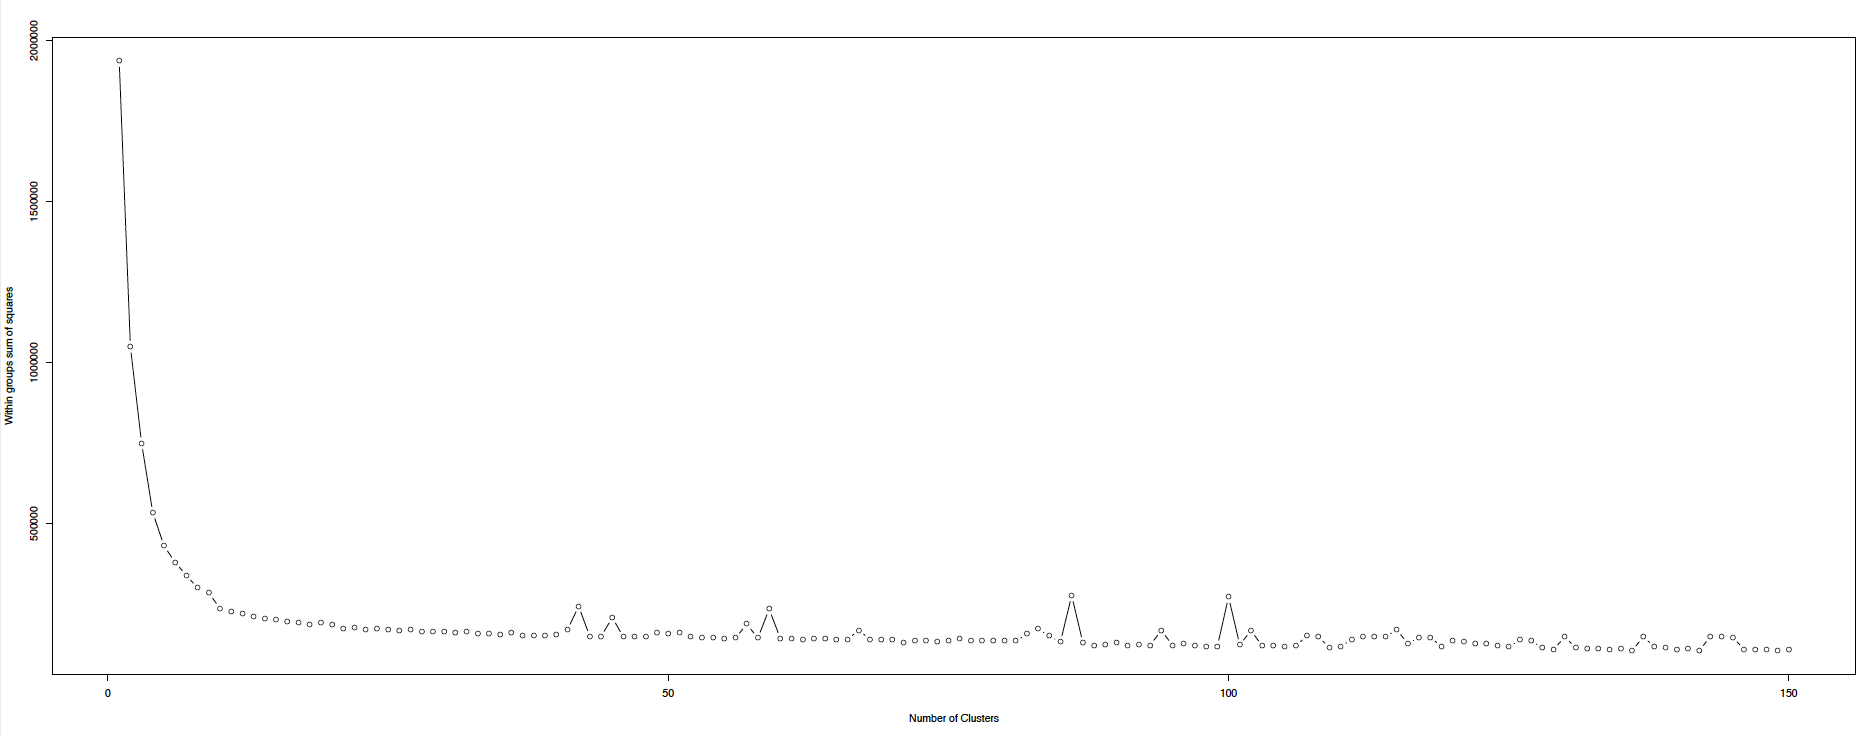
\includegraphics[width=0.95\textwidth]{Figures/Chapter4/kmeans/immgen_tcell_only_wssplot.png}
\caption{\small{An "elbow" plot showing how increasing the number of \textit{K} clusters results in a decrease in the overall within-module variance of the T cell data. The optimal value of \textit{K} is believed to sit at the point where adding additional clusters does not result in a substantial increase in the proportion of variance explained i.e. the "elbow" of the plot.} }
   \label{fig:18}
\end{figure}

\section{Distribution of ImmGen Coarse module genes within T cell K-means clusters}

For completeness we performed the same comparison of gene assignments between the ImmGen coarse modules and those produced by \textit{k}-means clustering, although given the small number of clusters resulting from the \textit{k}-means analysis, it is fair to say that this comparison is likely to be of limited value. Indeed, inspection of table 4.3 shows that \textit{k}-means module gene assignments are split across many of the ImmGen modules, providing further evidence that the clusters produced during the latest analysis of the T cell dataset do not represent modules of closely related gene expression profiles. It is possible that re-clustering of each \textit{k}-means module individually may result in better defined, more biologically relevant gene groups, but given that this algorithm clusters based purely on physical distances between data points, the results are unlikely to better those of more complex clustering methodologies such as WGCNA when it comes to the clustering of gene expression data.

\begin{landscape}
\small 
\begin{longtable}{|p{1.5cm}|p{1.25cm}|p{21cm}|}
\caption{Table detailing how genes assigned to each ImmGen Coarse module are dispersed within the modules generated by re-clustering of T cell samples with K-means}\\
\hline
ImmGen Coarse mod & Coarse mod size & Distribution of genes among K-means T cell data modules \\
\hline

1 & 334 & 2 (74) 7 (67) 4 (20) 3 (4) 1 (97) \\
2 & 229 & 3 (5) 2 (80) 1 (58) 7 (30) 4 (6) \\
3 & 344 & 7 (25) 2 (166) 3 (2) 1 (74) \\
4 & 118 & 3 (15) 2 (22) 4 (17) 6 (10) 7 (9) 1 (9) \\
5 & 313 & 2 (131) 1 (86) 7 (36) 3 (3) 4 (10) \\
6 & 111 & 7 (7) 1 (28) 2 (52) 4 (2) \\
7 & 30 & 2 (9) 1 (10) 4 (3) 7 (5) \\
8 & 23 & 1 (5) 2 (8) 4 (2) \\
9 & 15 & 1 (5) 2 (5) 7 (2) \\
10 & 14 & 1 (6) 7 (2) 2 (4) 4 (2) \\
11 & 153 & 1 (12) 2 (52) 7 (7) 8 (10) 4 (2) \\
12 & 46 & 2 (20) 1 (3) 7 (3) \\
13 & 101 & 2 (40) 7 (13) 1 (16) 4 (11) \\
14 & 73 & 2 (25) 7 (3) 1 (17) \\
15 & 38 & 2 (16) 7 (3) 1 (8) \\
16 & 363 & 2 (89) 1 (115) 7 (65) 4 (33) 3 (10) 6 (4) \\
17 & 201 & 1 (56) 3 (12) 4 (30) 7 (43) 6 (7) 2 (30) 5 (2) \\
18 & 146 & 7 (22) 2 (36) 1 (29) 4 (10) 3 (7) \\
19 & 125 & 1 (17) 2 (32) 3 (3) 4 (2) 7 (2) \\
20 & 54 & 3 (2) 1 (11) 2 (16) 7 (5) 6 (4) 4 (2) \\
21 & 82 & 2 (30) 7 (4) 1 (12) \\
22 & 39 & 2 (16) 1 (9) 7 (3) \\
23 & 54 & 7 (6) 2 (22) 1 (15) 4 (2) \\
24 & 486 & 2 (135) 1 (39) 7 (11) 4 (3) \\
25 & 438 & 2 (120) 1 (31) 7 (12) \\
26 & 247 & 1 (7) 2 (35) 7 (2) \\
27 & 72 & 2 (11) 1 (5) \\
28 & 55 & 1 (2) 2 (4) \\
29 & 37 & 2 (14) 1 (2) \\
30 & 76 & 2 (10) 1 (3) 7 (3) \\
31 & 40 & \\
32 & 101 & 2 (44) 1 (14) 7 (9) 4 (4) \\
33 & 147 & 2 (27) 7 (4) 1 (9) \\
34 & 117 & 1 (23) 2 (39) 4 (8) 7 (18) 3 (3) 6 (5) \\
35 & 268 & 2 (8) \\
36 & 202 & 2 (5) \\
37 & 41 & \\
38 & 42 & 2 (2) \\
39 & 45 & \\
40 & 67 & 2 (4) \\
41 & 54 & 2 (2) \\
42 & 53 & 2 (20) 1 (2) \\
43 & 46 & 2 (2) \\
44 & 118 & 7 (5) 2 (26) 1 (4) \\
45 & 315 & 2 (125) 1 (66) 7 (26) 4 (7) 3 (6) \\
46 & 155 & 2 (64) 1 (39) 4 (7) 7 (8) \\
47 & 134 & 2 (44) 7 (4) 1 (9) \\
48 & 134 & 7 (11) 2 (54) 1 (24) \\
49 & 108 & 2 (47) 1 (21) 7 (8) \\
50 & 91 & 2 (33) 1 (9) \\
51 & 51 & 2 (20) 1 (19) 4 (2) \\
52 & 149 & 4 (10) 7 (21) 2 (41) 1 (36) 3 (7) 6 (2) \\
53 & 97 & 1 (25) 2 (28) 7 (12) 4 (9) \\
54 & 38 & 2 (10) 4 (5) 1 (10) 7 (9) \\
55 & 26 & 2 (8) 1 (4) \\
56 & 71 & 2 (23) 1 (6) 4 (2) \\
57 & 64 & 2 (25) 1 (5) 7 (3) 4 (2) \\
58 & 55 & \\
59 & 15 & 2 (5) \\
60 & 19 & 2 (6) \\
61 & 45 & 2 (13) 1 (16) 7 (4) \\
62 & 62 & 2 (26) 1 (5) \\
63 & 37 & 1 (17) 2 (9) 7 (4) \\
64 & 26 & 1 (5) 2 (12) 3 (2) \\
65 & 37 & 2 (7) 1 (2) \\
66 & 21 & \\
67 & 19 & 1 (9) 7 (4) 2 (3) \\
68 & 14 & 2 (8) 1 (2) 7 (2) \\
69 & 22 & \\
70 & 13 & 2 (4) \\
71 & 19 & 2 (9) \\
72 & 13 & 2 (3) \\
73 & 12 & \\
74 & 15 & \\
75 & 12 & 1 (4) 2 (5) \\
76 & 15 & 2 (3) \\
77 & 11 & 2 (6) 1 (3) \\
78 & 18 & 1 (4) 2 (5) \\
79 & 7 & \\
80 & 56 & 2 (6) 6 (3) \\
81 & 211 & 7 (9) 1 (16) 2 (33) 3 (2) \\


\hline
\end{longtable}
\end{landscape}

\section{Conclusions and Future Work}

Here we present the results of re-clustering of T cell data from the publicly available ImmGen resource. WGCNA, Hclust and \textit{K}-means were all applied to this dataset with surprisingly varied results. Indeed, while WGCNA and Hclust produced many gene modules, \textit{K}-means clustering delivered only a handful. It is believed that this latter result is due to the fact that in \textit{K}-means clustering, no account is taken of the correlations between samples. In a biological context, correlation analysis is one of the key ways in which we can determine the relationship between genes in a given setting and so to ignore these connection seems rather counter intuitive. We therefore suggest that \textit{K}-means is not an appropriate choice for the clustering of large gene expression datasets. This work also highlights the need for the establishment of comprehensive and user-friendly module annotation and qualitative assessment techniques. Without these, it is not feasible to attempt detailed annotation of such large module lists and so we can not truly evaluate the above clustering results at this time.




